\chapter{Bomba Kryptologiczna}
%% https://www.cryptocellar.org/pubs/ukwa.pdf%%
%% https://www.cryptocellar.org/enigma/files/rejewski-paper.pdf %%

% FOR SUPPLIED INTELLEGENCE SEE
% https://archive.org/details/enigmahowgermanm0000koza/page/16/mode/2up
% - Page 16 %
Rejewski was saddled with arguably the most complex discoveries in
Enigma code breaking. Not only did he need to determine a means to
recover daily keys from limited intellegence supplied by ?? but he
additionally needed to recover the wirings of the rotors themselves.
\section{Characteristics}
Rejewksi quickly determined the protocol by which messages were
enciphered -- in fact, he stated the this protocol was ``obvious.''
We will see that purely with knowledge of this procudure and some
military intellegence, Rejewski was able to determine the rotor
wirings necessary to make further cryptanalysis possible.
\\\\Consider the first six letters transmitted according to our
encryption producedure. Operator Alice has some three letter private
key (say \texttt{XYZ}) which she encodes twice with the machine
settings specified by her key sheet. This will give us six encrypted
letters
$\sigma_1(\texttt{X})\sigma_2(\texttt{Y})\sigma_3(\texttt{Z})\sigma_4(\texttt{X})\sigma_5(\texttt{Y})\sigma_6(\texttt{Z})$.
Suppose these six letters are given as
\begin{center}
	\texttt{ABC} \texttt{DEF}
\end{center}
That is
\begin{align*}
	\sigma_1(\texttt{X}) & = \texttt{A} \\
	\sigma_2(\texttt{Y}) & = \texttt{B} \\
	\sigma_3(\texttt{Z}) & = \texttt{C} \\
	\sigma_4(\texttt{X}) & = \texttt{D} \\
	\sigma_5(\texttt{Y}) & = \texttt{E} \\
	\sigma_6(\texttt{Z}) & = \texttt{F} \\
\end{align*}
Since each $\sigma_i$ is represented by 13 disjoint transpositions we
can deduce, for example, that
\[
	\sigma_1\sigma_4(D) = \sigma_1(X) = A.
\]
With a sufficient set of hexagrams from gathered messages, we could
then fully deduce the permutation $\sigma_1\sigma_4$. Further, we
could recover $\sigma_2\sigma_5$ and $\sigma_3\sigma_6$. Rejewski
refered to these paired permutations as {\bf{characteristics}}. In
practice, such recovered characteristics may look like
\begin{align*}
	\sigma_1\sigma_4 & =
	(\texttt{DVPFKXGZYO})(\texttt{EIJMUNQLHT})(\texttt{BC})(\texttt{RW})(\texttt{A})(\texttt{S})
	\\
	\sigma_2\sigma_5 & =
	(\texttt{BLFQUEOUM})(\texttt{HJPSWIZRN})(\texttt{AXT})(\texttt{CGY})(\texttt{D})(\texttt{K})
	\\
	\sigma_3\sigma_6 & = (\texttt{ABVIKTJGFCQNY})(\texttt{DUZREHLXWPSMO})
\end{align*}
Rejewski noted a key structural similarity between all such
characteristics recovered in this fashion: in each characteristic,
cycles of the same length appear in pairs.
\\\\To see why this happens consider the following lemma,
\begin{lemma}
	\label{cillies}
	Suppose $(\alpha\beta)$ appears in $\sigma_i$ for $i\in\{1,2,3\}$.
	Then $\alpha$ and $\beta$ will appear in disjoint cycles of
	$\sigma_i\sigma_{i+3}$ of equal length.
\end{lemma}
\begin{proof}
	%% chrome-extension://efaidnbmnnnibpcajpcglclefindmkaj/https://www.math.ias.edu/files/wam/rejewski.pdf
	% %%
	We begin by noting that if $(\alpha\beta)$ is in $\sigma_{i+3}$
	then $\pi$ contains fixed points at $\alpha$ and $\beta$ and our
	claim is true. Then without loss of generality we can arrange
	$\sigma_{i}$ and $\sigma_{i+3}$ (non-exhaustively) in the following way:
	\[
		\setlength{\arraycolsep}{15pt}
		\begin{array}{cc}
			\sigma_i      & \sigma_{i+3} \\
			\hline
			(\alpha\beta) & (\beta x_1)  \\
			(x_1 x_2)     & (x_2 x_3)    \\
			\vdots        & \vdots       \\
			(x_{k-1} x_k) & (x_k \alpha)
		\end{array}
	\]
	Then the product $\sigma_i\sigma_{i+3}$ will be
	\[
		\sigma_1\sigma_{i+3} = (\alpha x_1 x_3 \dots x_{k-1} )(x_k
		x_{k-2} \dots x_2 \beta)
	\]
	and thus $\alpha$ and $\beta$ end up in disjoint cycles of equal length.
\end{proof}

This lemma has several consequences.
\begin{itemize}
	\item A characteristic like $\sigma_1\sigma_4$ which has two
	      singletons $\texttt{A}$ and $\texttt{S}$ then both $\sigma_1$ and
	      $\sigma_4$ must have the transposition $(\texttt{AS})$.
	\item A characteristic like $\sigma_3\sigma_6$ (two disjoint 13
	      cycles) reduces the space of possible $\sigma_3$'s to just 13
	      permutations which will take the form
	      \begin{center}
		      $(\texttt{AD})(\texttt{BO})(\texttt{VM})\dots(\texttt{YU})$ \\
		      $(\texttt{AU})(\texttt{BD})(\texttt{VO})\dots(\texttt{YZ})$ \\
		      $\vdots$                                       \\
		      $(\texttt{AO})(\texttt{BM})(\texttt{VS})\dots(\texttt{YD})$
	      \end{center}
	      and similarly for $\sigma_6$.
\end{itemize}
Thus with absolutely no knowledge of the rotor wirings or the daily
key, we can already tractibly compute a searchable space of
$\sigma_i$'s. To determine which $\sigma_i$ is the correct one, we
make use of the most prevalent bug in cryptography -- operator error.

\subsection{Cillies}\label{cillies}
Enigma operators were instructed to construct random trigrams for
their message keys -- likely to prevent frequency analysis attacks on
the hexagrams beginning messages; However, operators often chose the
same trigrams for each message. Some examples might inclide
\begin{itemize}
	\item Initials or first letters of the operator's spouse. For
	      example, \texttt{CIL} perhaps deriving from the name ``Cecelia''
	      being shortened to ``cillie''. Allegadely for this reason, poor
	      selections of trigrams from operators became known as {\bf{cillies}}.
	\item The same letter encoded three times such as \texttt{JJJ}
	\item Locations such as \texttt{LON} representing London.

	      %% Battle of wits the complete story of codebreaking in World War
	      % II PAGE 143 %%
\end{itemize}
By keeping track of various radio stations which used cillies.
Rejewski had a reasonable guess as to what the message key used for a
particular ciphertext were. Suppose we recieved three hexagrams
originating from a radio station which often used \texttt{JJJ} as
their message key:
\begin{center}
	\texttt{SUG SMF}\\
	\texttt{SJM SPO}\\
	\texttt{SYX SCW}.
\end{center}

We can then compare these message keys against our possibilites for
$\sigma_i$s to determine if $\texttt{JJJ}$ could have in fact been
used to encipher these hexagrams. For example, the first hexagram
could not have been used since \texttt{J} and \texttt{G} lie in the
same cycle of $\sigma_3\sigma_6$ which would contradict lemma
\ref{cillies}. Contiuing in this fashion we may hypothesize that the
third hexagram was likely an enciphering of the repeated letter $\texttt{J}$.
\\\\To confirm this hypothesis we can use the supposition to further
reduce the possible $\sigma_i$s. In fact, in our case, such a
hypothesis would completely determine which $\sigma_3$ and $\sigma_6$
were being used and for the remaining $\sigma_i$s we are only left
with a small set of options. We can then confirm our hypothesis by
trying such $\sigma_i$s on hexagrams from other radio stations
suspected of using cillies. If we find that $\texttt{PPP}$ is the
message key corresponding to our deduced $\sigma_i$s we have reason
to believe that our initial hypothesis was correct. If our hexagram
corresponded to a key \texttt{PPA} we may only need to select a new
choice of possible $\sigma_i$s to instead produce the expected cilly.
In this way, we can recover each $\sigma_i$ and thus recover any
transmission's message key -- all without any knowledge of internal
wirings, plugboard settings, or daily keys.
\section{Wiring Recovery}

Equipped with a means to determine each $\sigma_i$, Rejewski set
himself to finding the internal wirings of the rotors. The full
recovery of rotor wirings and turovers is out of scope of this paper;
However, we will provide a brief description to illustrate that with
minimal intellegence information, entire rotor wirings were able to be deduced.
\\\\We begin by expanding $\sigma_i$ to
\[
	\sigma_i = S^{-1}P^{-(x+i)}N^{-1}P^{x+i}M^{-1}L^{-1}RLMP^{-(x+i)}NP^{x+i}S
\]
where $x$ accounts for the initial starting position of the rightmost rotor.
Since $M^{-1}L^{-1}RLM$ does not change between $\sigma_i$s we will
denote this permutation $Q$ thus simplifying our earlier expression to
\[
	\sigma_i = S^{-1}P^{-(x+i)}N^{-1}P^{x+i}QP^{-(x+i)}NP^{x+i}S
\]
Rejewski knew the plugboard settings for two whole months, so he
began shifting knowns and unknowns to opposite sides. Shifting things
around gives us
\begin{align*}
	                    & \sigma_i = S^{-1}P^{-(x+i)}N^{-1}P^{x+i}QP^{-(x+i)}NP^{x+i}S \\
	\Rightarrow\text{ } & S\sigma_i S^{-1} =
	P^{-(x+i)}N^{-1}P^{x+i}QP^{-(x+i)}NP^{x+i}
	\\
	\Rightarrow\text{ } & P^{(x+i)}S\sigma_i S^{-1}P^{-(x+i)} =
	N^{-1}P^{x+i}QP^{-(x+i)}N
\end{align*}
To further simplify notation we will then define ${\rho_i} \coloneq
	P^{(x+i)}S\sigma_i S^{-1}P^{-(x+i)}$. Then we have now have
\[
	\rho_i = N^{-1}P^{x+i}QP^{-(x+i)}N
\]
where $\rho_i$s are known from the key sheets Rejewski had access to.
We will now eliminate this equations dependence on $Q$ by considering
pairs of $\rho_i$ and $\rho_{i+1}$
\begin{align*}
	\rho_i\rho_{i+1} & = N^{-1}P^{x+i}QP^{-(x+i)}NN^{-1}P^{x+i+1}QP^{-(x+i+1)}N \\
	                 & = N^{-1}P^{x+i}QP^{-(x+i)}P^{x+i+1}QP^{-(x+i+1)}N        \\
	                 & = N^{-1}P^{x+i}QPQP^{-(x+i+1)}N                          \\
	                 & =N^{-1}P^{x+i}(QPQP^{-1})P^{-{x+i}}N
\end{align*}
Each $\rho_i\rho_{i+1}$ shares the common subexpression $QPQP^{-1}$.
We can eliminate this subexpression by noting
\begin{align*}
	\rho_{i+1}\rho_{i+2} & = N^{-1}P^{x+i+1}(QPQP^{-1})P^{-{x+i+1}}N
	\\
	                     & =
	N^{-1}P^{x+i+1}(P^{-(x+i)}NN^{-1}P^{x+i})(QPQP^{-1})(P^{-(x+i)}NN^{-1}P^{x+i})P^{-{x+i+1}}N
	\\
	                     & =
	N^{-1}P^{x+i+1}P^{-(x+i)}N(N^{-1}P^{x+i}QPQP^{-1}P^{-(x+i)}N)N^{-1}P^{x+i}P^{-{x+i+1}}N
	\\
	                     & =
	N^{-1}P^{x+i+1}P^{-(x+i)}N(\rho_i\rho_{i+1})N^{-1}P^{x+i}P^{-{x+i+1}}N
	\\
	                     & = N^{-1}P^{-1}N(\rho_i\rho_{i+1})N^{-1}PN
	\\
\end{align*}
We now have a relationship between each $\rho_i\rho_{i+1}$ and
$\rho_{i+1}\rho_{i+2}$ by conjugating by $N^{-1}PN$. Now recall from
theorem %\ref{IDK}% that if $\rho_i\rho_{i+1}$ has a reasonbaly large
% cycle structure, then there are only a limited number of possible
% permutations for $N^{-1}PN$. The relationship between
% $\rho_{i+1}\rho_{i+2}$ and $\rho_{i+2}\rho_{i+3}$ will further
% reduce these possibilities since of course $N^{-1}PN$ must be the
% same between these two relationships. Eventually, we can fully
% deduce $N^{-1}PN$. Finally, this will give us $26$ possibilites for
% $N$ representing its $26$ intial starting positions, and thus we
% can recover $N$ itself representing the internal wiring of the
% rigthmost rotor.
\\\\In a similar fashion we can recover the remaining rotor wirings
though often with the help of other mathematical tricks, not to
mention military intellegence and luck. From this point forward, we
will assume that the cryptanalyst now has access to the wirings of
all the rotors as well as the reflector.

\section{The Grill Method}

We now have deduced all of the rotors $N$, $M$, $L$, $R$ and each
$\sigma_i$. We will use this information to recover the daily keys.
For the moment, let us assume $S$ is the identity permutation. Then
rearranging $\sigma_i$ we get
\begin{align}
	Q = P^{-(x+i)}NP^{x+i}\sigma_iP^{-(x+i)}N^{-1}P^{x+i} \label{eq:q_eq}
\end{align}
Since $Q$ must be the same for each such equation involving
$\sigma_i$ we will devise a manual way to deduce $Q$. We can
precompute $N$, $P^{-1}NP$, $\dots$, $P^{4}NP^{-4}$ and arrange them
in a large sheet called the {\bf{bottom sheet}}.
Then for each $\sigma_i$ we can write out $\sigma_i$ with a slit
beneath it to allow space for each possible $P^{-k}NP^k$. We will
illustrate this for $\sigma_1$ and denote the spaces beneath with periods.
\begin{align*}
	\texttt{|}          & \texttt{ABCDEFGHIJKLMNOPQRSTUVWXYZ} \texttt{|} \\
	\sigma_1\texttt{ |} & \texttt{SRWIVHNFDOLKYGJTXBAPZECQMU} \texttt{|} \\
	\texttt{|}          & \texttt{..........................} \texttt{|}
\end{align*}
We will call this the {\bf{top sheet}}. By sliding the bottom sheet
beneath the top sheet we can test various values of $P^{-k}NP^{k}$ to
see what values of $Q$ they give. For example, for $k = 0$ we have
\begin{align*}
	\texttt{|}          & \texttt{ABCDEFGHIJKLMNOPQRSTUVWXYZ} \texttt{|} \\
	\sigma_1\texttt{ |} & \texttt{SRWIVHNFDOLKYGJTXBAPZECQMU} \texttt{|} \\
	N \texttt{ |}       & \texttt{KJPZYDTIOHXCSGUBRNWFMVEQLA} \texttt{|}
\end{align*}
We know that $Q(\texttt{A}) =
	(P^{-k}NP^k)\sigma_i(P^{-k}NP^k)^{-1}(\texttt{A})$. Therefore to compute
$Q(\texttt{A})$ we first begin at $\texttt{A}$ in our bottom row to
find that $N^{-1}(\texttt{A})=\texttt{Z}$. We now map $\texttt{Z}$
through $\sigma_i$ by finding $\texttt{Z}$ on the top row and seeing
where it lands in the middle row, thus giving
$\sigma_iN^{-1}(\texttt{A}) = \texttt{U}$. Finally to see where $N$
maps $\texttt{U}$ by finding $\texttt{U}$ on the top row and seeing
where it lands in the middle row, thus giving $Q(\texttt{A}) =
	N\sigma_iN^{-1}(\texttt{A}) = M$. Continuing in this fashion we can
get a candidate $Q$ generated by the guess that $\sigma_i$ aligned
with $N$ in the sheet. Recall that $Q$ must be consistent between
each equation \ref{eq:q_eq}. To check this we can simply construct
our top sheet so that each $\sigma_i$ is placed over one another each
with a slot beneath it. We can now get candidate $Q$s for each
$\sigma_i$. If we find that our offset of the bottom sheet creates
inconsistencies we can move the bottom sheet up by one until we find
candidates that are consistent between each $\sigma_i$.
\\\\If $S$ were truly the identity then we would ultimately find an
offset that generates identical $Q$s for each $\sigma_i$. Of course,
$S$ will not be the identity. Thus, instead of looking for perfect
consistency between each $Q$ we are only looking for relative
consistency between each $Q$ where perhaps a majority send one letter
to another. By comparing $Q$s generated by each $\sigma_i$ we can
deduce with reasonable certainty the value of the true $Q$ by just
considering where the majority of the $Q$s map \texttt{A},
\texttt{B}, and so on. Further, the offset in the bottom sheet which
generated the most consistent permutations $Q$ will give us the
absolute position of the rightmost rotor. Additionally, using this
method, we can see where the $Q$s fail to line up to determine which
letters are steckered and which are unsteckered, along with some of
the steckerings themselves. Such a method was called the {\bf{grill
			method}} and required tedious work and had many possibilites for mistakes.
\\\\To determine the absolute positions of the remaining two rotors
we can simply enumerate all $26^2 = 676$ positions of the left two
rotors (for both possible orderings of the rotors) until $Q$ is
produced. In practice, a catalogue was eventually compiled which
associated each $Q$ to a corresponding position and ordering of the
left two rotors. Now equipped with each absolute rotor position, we
still must determine the ring settings.
\\\\To determine the ring settings we make use of another operator
error. Often messages began with the letters \texttt{ANX} which is
the German word ``to'' along with \texttt{X} denoting a space. We
could therefore set the ring setting to its default location and then
brute force all $26^3$ possible rotor positions until the first
letters in the deciphered message were \texttt{ANX}. Once we knew the
absolute position at which this occured, along with the message key,
we can immediately determine what the ring settings must have been to
produce this message -- since the ring setting and rotor position
have inverse effects on the rotor permutation.
\\\\One key point regarding the grill method is that at the time when
it was in use only $3$ jacks were used in the plugboard. This means
that the $Q$s generated by each $\sigma_i$ were relatively similar
since the permutation $S$ had less impact on average. However, the
Germans eventually used up to $10$ jacks making the grill method
infeasible since we can no longer determine confidently the true
value of $Q$. This fact will later necessitate the development of an
additional tool called the {\bf{Bomba}} later discussed in this chapter.

\section{The Clock Method}\label{clock_method}

At this point Rejewski and his team were able to recover daily keys,
but the above methods are extremely slow and inefficient. Many
optimizations were made over the years. We will now examine one
particular optimization.
\\\\While we do know the wirings of the rotors, we do not know when
we begin our cryptanalysis what the order of these rotors were. At
the time there were only three rotors in use (\texttt{I},
\texttt{II}, \texttt{III}) so one could simply try all 3 rotors as
the rightmost one and repeat the above analysis. Of course, this
makes the above method 3 times slower. In practice, early Enigma
daily keys kept rotor positions the same for an entire 3 month period
meaning this analysis did not need to be done too frequently.
\\\\However, Jerzy Różycki worked out an efficient method to
determine the rightmost rotor which he called the {\bf{clock
			method}}. The clock method attempted to determine where the turnover
notch was for the rightmost rotor. From this we could immediately
determine which of the three rotors was used.

\subsection{Index of Coincidence}\label{ioc}
In a string of random text from a 26 letter alphabet we get a uniform
distribution of letters. Thus we expect each letter to appear with a
$\frac{1}{26}$ probability. When we align two pieces of random text,
it then follows that we expect $1$ letter to match up between them
every $26$ letters. However, text which encodes a language does
not generate a uniform distribution. Distributions for various
languages have been well studied and are the information needed for
frequency analysis. Having a non-uniform distribution also implies
that when we align two pieces of text which encode a language, the
chance that a letter from the first piece of text will align at the
same position with a letter
from the second piece of text is non-uniform, this distribution is
called the {\bf{index of coincidence}}. In particular, for German, we
find that the expected number of alignments (called
	{\bf{coincidences}}) between two pieces of text $26$ letters long is
$2.05$. If these texts
%https://en.wikipedia.org/wiki/Index_of_coincidence% It then follows
% that if two pieces of text
are enciphered with the \emph{same} polyalphabetic cipher, we expect
to see the same distribution of coincidences. If they are enciphered
with \emph{different} polyalphabetic ciphers, we expect to return to
a uniform distribution.
\\\\To make use of this property, we can select two messages with
message keys (determined as in section~\ref{cillies}) whose first two
letters coincided (e.g. \texttt{XYA} and
\texttt{XYF}). This meant that both messages were encoded with the
only difference being in their rightmost rotor. If at some point
during encoding the first message, its rotors align with the rotors
used to encode the second message, we would expect to see the number
of coincidences between the messages to suddenly spike significantly,
in this way, we can detect when the two messages had their rotors
align. This does not work, however, if turnover occurs. In that case, the two
messages will not align in their rotor positions and we will see a
random distribution of coincidences. If we align the message
generated by $\texttt{XYA}$ on top of the message generated by
$\texttt{XYF}$ we can slide the bottom message until is 5 positions
further than the top message,
\begin{align*}
	 & \texttt{XYA}: \texttt{PASLK XASSP AUSDK XPVNW UULVT LWKRE KGUQO
		DSUKV ZOLMZ ZHYBF}
	\\
	 & \texttt{XYF}: \texttt{ }\texttt{ }\texttt{ }\texttt{ }\texttt{
	}\texttt{ }\texttt{BAWXV ETTOP JZHXL VWGGQ MWDII OEHQO YSLRB IYLGB
		CHBYT }
	\\
	 &
	\ \ \ \ \ \ \ \ \ \ \ \ \ \ \ \ \ \ \texttt{*}\ \ \ \ \ \ \ \ \ \ \ \ \ \ \ \ \ \ \ \ \ \ \ \ \ \ \ \ \ \ \ \ \ \ \ \ \ \texttt{*}\ \ \ \ \ \ \ \ \ \ \ \texttt{**}\ \ \ \texttt{*}\ \ \ \ \ \ \ \ \ \texttt{*}\ \ \ \ \ \ \ \texttt{*}
\end{align*}
at this point we would expect the texts to both be encoded by
$\texttt{XYF}$ and the number of coincidences (indicated by
\texttt{*}) should spike as we see in the above diagram. Given that
this occured, this means no turnover occured between $\texttt{A}$ and
$\texttt{F}$. This, for example, eliminates rotor \texttt{II} as a
candidate since its turnonver occurs when \texttt{E} is displayed in
the window. We can gain further information by performing the above
procecdure but now with the message encoded by $\texttt{XYF}$ on the
top and the message encoded by $\texttt{XYA}$ on the bottom. In this
way we can determine which rotor was being used. The clock method was
a precursor to a method we will discuss later known as Banburismus.
The important takeaway is that, while language frequency analysis may not be
strong enough to decode Enigma messages, it may be strong enough to
determine elements of the key like rotor choice or ordering.

\section{The Cyclometer}

These manual methods of decryption became increasingly difficult as
German operators were instructed to use more plugboard jacks and
increased the rate at which daily keys changed. Rejewski wanted to
produce a mechanical means of performing a similar deduction. He
returned to the characteristics associated with a particular day's
key. He noticed that the cycle structure of a characteristic did not
regularly repeat (if at all). Then we perhaps could create a
``fingerprint'' of a key by noting the cycle structure of all three
characteristics associated to the key. Now that Rejewski had the
internal rotor wirings, he could build a machine that could
immediately produce the cycle structure of characteristics for a given setting.
\\\\Let us first understand the manual implementation of such a
deduction. Assuming an identity plugboard $S$ we can use our internal
rotor wirings to know the exact permutaition $\sigma_1$ and
$\sigma_4$ for any initial rotor position. In specific, suppose we have

\begin{center}
	\[
		\left(
		\begin{array}{llllllllllllllllllllllllll}
				\texttt{A} & \texttt{B} & \texttt{C} & \texttt{D} &
				\texttt{E} & \texttt{F} & \texttt{G} & \texttt{H} &
				\texttt{I} & \texttt{J} & \texttt{K} & \texttt{L} &
				\texttt{M} & \texttt{N} & \texttt{O} & \texttt{P} &
				\texttt{Q} & \texttt{R} & \texttt{S} & \texttt{T} &
				\texttt{U} & \texttt{V} & \texttt{W} & \texttt{X} &
				\texttt{Y} & \texttt{Z}                             \\
				\texttt{P} & \texttt{T} & \texttt{K} & \texttt{X} &
				\texttt{R} & \texttt{Z} & \texttt{Q} & \texttt{S} &
				\texttt{W} & \texttt{M} & \texttt{C} & \texttt{O} &
				\texttt{J} & \texttt{Y} & \texttt{L} & \texttt{A} &
				\texttt{G} & \texttt{E} & \texttt{H} & \texttt{B} &
				\texttt{V} & \texttt{U} & \texttt{I} & \texttt{D} &
				\texttt{N} & \texttt{F}
			\end{array}
		\right)
	\]
	$\sigma_1$
\end{center}
\begin{center}
	\[
		\left(
		\begin{array}{llllllllllllllllllllllllll}
				\texttt{A} & \texttt{B} & \texttt{C} & \texttt{D} &
				\texttt{E} & \texttt{F} & \texttt{G} & \texttt{H} &
				\texttt{I} & \texttt{J} & \texttt{K} & \texttt{L} &
				\texttt{M} & \texttt{N} & \texttt{O} & \texttt{P} &
				\texttt{Q} & \texttt{R} & \texttt{S} & \texttt{T} &
				\texttt{U} & \texttt{V} & \texttt{W} & \texttt{X} &
				\texttt{Y} & \texttt{Z}                             \\
				\texttt{J} & \texttt{W} & \texttt{V} & \texttt{R} &
				\texttt{O} & \texttt{S} & \texttt{U} & \texttt{Y} &
				\texttt{Z} & \texttt{A} & \texttt{T} & \texttt{Q} &
				\texttt{X} & \texttt{P} & \texttt{E} & \texttt{N} &
				\texttt{L} & \texttt{D} & \texttt{F} & \texttt{K} &
				\texttt{G} & \texttt{C} & \texttt{B} & \texttt{M} &
				\texttt{H} & \texttt{I}
			\end{array}
		\right)
	\]
	$\sigma_4$
\end{center}
Then to find the permutation $\sigma_1\sigma_4$ we might do the
following. We begin with \texttt{A}. We first run \texttt{A} through
$\sigma_4$ to get \texttt{J}. We then run \texttt{J} through
$\sigma_1$ to get \texttt{M}. Thus we see
$\sigma_1\sigma_4(\texttt{A}) = \texttt{M}$. Now we would continue
with \texttt{M} sending it back into $\sigma_4$. Eventually after
jumping back and forth between $\sigma_1$ and $\sigma_4$ we we will
have encountered all letters contained in the same cycle as
\texttt{A}. We do, however, encounter some other letters as well.
This method is effectively the same method used in lemma
\ref{cillies} to find the two disjoint cycles of equal length
produced in a characteristic. In fact, by switching back and forth
between $\sigma_1$ and $\sigma_4$ we will find alternating elements
of the pair of cycles of equal length which contain \texttt{A}. We
can mechanize this process via the following
circuit\footnote{Throughout this paper, diagrams will represent a
	simplified Enigma machine consisting of only four letters
	(\texttt{A},\texttt{B}, \texttt{C}, and \texttt{D}):}
\begin{center}
	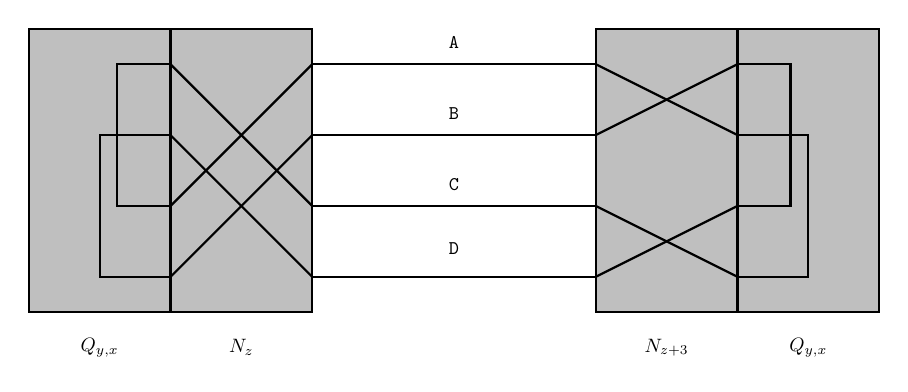
\begin{tikzpicture}[thick, scale=0.9, every node/.style={scale=0.7}]
		% Draw the box
		\draw[fill=lightgray] (2-5,-1.5-1) rectangle (4-5,2.5-1) node[midway] {};

		\node at (3-5, -2-1) {$Q_{y,x}$};

		\draw[-] (2-3, 2-1) |- ++(-0.75, 0) |- (2-3, 0-1);
		\draw[-] (2-3, 1-1) |- ++(-1, 0) |- (2-3, -1-1);

		\draw[fill=lightgray] (2-3,-1.5-1) rectangle (4-3,2.5-1) node[midway] {};

		\node at (3-3, -2-1) {$N_z$};

		% Draw the lines inside the box to represent the mapping
		\draw[-] (2-3, 2-1) -- (4-3, 0-1);
		\draw[-] (2-3, 1-1) -- (4-3, -1-1);
		\draw[-] (2-3, 0-1) -- (4-3, 2-1);
		\draw[-] (2-3,-1-1) -- (4-3, 1-1);

		% Draw the lines inside the box to represent the mapping
		\draw[-] (2-1, -1-1) -- (4+3, -1-1);
		\draw[-] (2-1, 0-1) -- (4+3, 0-1);
		\draw[-] (2-1, 1-1) -- (4+3, 1-1);
		\draw[-] (2-1,2-1) -- (4+3, 2-1);

		\draw[fill=lightgray] (2+3,-1.5-1) rectangle (4+3,2.5-1) node[midway] {};

		\node at (3+3, -2-1) {$N_{z+3}$};

		% Draw the lines inside the box to represent the mapping
		\draw[-] (2+3, 1-1) -- (4+3, 2-1);
		\draw[-] (2+3, 2-1) -- (4+3, 1-1);
		\draw[-] (2+3, 0-1) -- (4+3, -1-1);
		\draw[-] (2+3,-1-1) -- (4+3, 0-1);

		\draw[fill=lightgray] (2+5,-1.5-1) rectangle (4+5,2.5-1) node[midway] {};

		\node at (3+5, -2-1) {$Q_{y, x}$};

		\draw[-] (2+5, 2-1) |- ++(0.75, 0) |- (2+5, 0-1);
		\draw[-] (2+5, 1-1) |- ++(1, 0) |- (2+5, -1-1);

		\node at (2+1, 2.3-1) {$\texttt{A}$};
		\node at (2+1, 1.3-1) {$\texttt{B}$};
		\node at (2+1, 0.3-1) {$\texttt{C}$};
		\node at (2+1, -0.6-1) {$\texttt{D}$};

	\end{tikzpicture}
\end{center}

In this circuit $N_z$ represents the rightmost rotor at some position
$z$ and $Q_{y,x}$ represents our fictious rotor (consisting of $M$,
$L$, and $R$) at a fixed position $y$ and $x$ -- we will denote this
position $(x,y,z)$. Note that right hand
rotor in the permutation depicted on the right is 3 steps further
than the right hand rotor depicted on the left. When we now apply a
current at \texttt{A} the current will travel back and forth through
$N^{-1}_zQ_{y,x}N_z$ and $N^{-1}_{z+3}Q_{y,x}N_{x+3}$ and reach all
the letters contained
in the pair of cycles of equal length which contain \texttt{A}, that
is, the number of wires electrified is double the length of the cycle
containing \texttt{A}. If we connect each wire to a bulb, we can
count the number of illuminated bulbs and can quickly determine the length of
the cycles in a permutation $\sigma_1\sigma_{4}$ at any given
position of rotors $(x,y,z)$. We can now rotate through all
$26^3$ positions of the rotors and create a catalogue of all
characteristics $\sigma_1\sigma_3$ (note that $\sigma_2\sigma_5$ and
$\sigma_3\sigma_6$ can be retrieved by just looking at the next two
catalogue entries). We must also consider all 6 orderings of rotors
\texttt{I}, \texttt{II}, and \texttt{III}. Thus we can laboriously
generate a catalogue of all rotor orders and settings consisting of
$6\cdot 26^3 = 105456$ entries.
\\\\Now equipped with this catalogue, the cryptanalyst could use the
traffic from a given day to determine the characteristics, look up
the cycle types in the catalogue, and determine the rotor order and
absolute rotor positions. The plugboard settings could then be
determined by comparing the characteristics recovered from the
traffic against the characteristics generated by the discovered rotor
positions with no plugboard jacks inserted. Finally the ring position
could be recovered as discussed before by using known plaintext from
the message. This ultimately reduced the time to find a day's
settings to roughly $15$ minutes.
\\\\Note that the machine made finding cycles in permutations
instantaneous by connecting each cycle in its own disjoint electrical
circuit. This first attempt at mechanizing the process of decryption
is a very early predacessor to the primary topic of this paper, the
Bombe. This method of enumerating cycles, as we will see, is the core
of the Bombe's primary function.
\section{The Bomba}

As mentioned prior, the addition of plugboard jacks made the grill
method infeasible.
Further, beginning on September 15, 1938, the German military changed
the protocol by which Enigma messages were encoded, making the grill
method completely obsolete. A new means of fingerprinting messages
outside of characteristics needed to be developed. Further, compared
to the grill method, such a new method would need to account for the
fact that the plugboard swapped many more letters.

\subsection{Changes to the Enigma Protocol}

%% https://www.ciphermachinesandcryptology.com/en/enigmaproc.htm %%
%% https://www.tandfonline.com/doi/full/10.1080/01611194.2010.486257?journalCode=ucry20
% &&
Starting in 1938, the German key sheets began removing an explicit
window setting (\emph{Grundstellung}) and added an indicator group
known as the \emph{Kenngruppen}. The indicator group was an extra
identification added to messages to note which key was being used. It
serves no cryptographic purpose so we will just discuss the way in
which the message key was obtained.
\\\\Operators were now instructed to choose a random window setting
(\emph{Grundstellung}) for each message. The operator then sent the
window setting in plaintext and proceeded to encode their message key
(\emph{Spruchschlüssel}) twice, enciphered with the chosen window
setting. % \begin{figure}[h]
%   \begin{center}
%     \resizebox{0.98\textwidth}{!}{
%       \begin{tabular}{|c|c|c|c|c|}
%         \hline
%         \textbf{\emph{\texttt{Datum}}}               &
%         \textbf{\emph{\texttt{Walzenlage}}}          &
%         \textbf{\emph{\texttt{Ringstellung}}}        &
%         \textbf{\emph{\texttt{Steckerverbindungen}}} &
%         \textbf{\emph{\texttt{Kenngruppen}}}
%                                                                                               \\
%         \hline
%         \texttt{31.}                                 & \texttt{I II
% V}          & \texttt{10 14 02} & \texttt{BF SD AY HG OU QC WI RL}
% & \texttt{sfy azy zkq bqi} \\
%         \texttt{30.}                                 & \texttt{V IV
% I}          & \texttt{04 25 01} & \texttt{UE PL
%         AY TB ZH WM OJ DC}                           & \texttt{iuy
% swz omo myj}
%                            \\
%         \texttt{29.}                                 & \texttt{III
% V II}        & \texttt{13 11 06} & \texttt{WJ VD
%         PO MQ FX ZR NE LG}                           & \texttt{rui
% kao fqi rwu}
%                            \\
%         \texttt{28.}                                 & \texttt{I
% III II}        & \texttt{09 16 12} & \texttt{HR
%         TJ LD IO CN GX QK PZ}                        & \texttt{ioy
% kjv yko fpz}
%                            \\
%         $\vdots$                                     & $\vdots$
%             & $\vdots$          & $\vdots$
% & $\vdots$                 \\
%         \hline
%       \end{tabular}}
%   \end{center}
%   \caption{Mock Enigma Key Sheet for 1938}
%   \label{fig:keysheet_bomba}
% \end{figure}
% %chrome-extension://efaidnbmnnnibpcajpcglclefindmkaj/https://www.tandfonline.com/doi/pdf/10.1080/01611190802562809%
% \\From the keysheet, the operator chose a trigram from the day's
% indicator groups. Then by adding two random letters to the trigram,
% they would generate a hexagram called a
% \emph{Buchstabenkenngruppe}. For example on the date of the 29th in
% figure \ref{keysheet_bomba}, the operator might choose the second
% indicator group to get a \emph{Buchstabenkenngruppe} of
% \texttt{LOKAO}. When sending a message the operator was to send a
% message with the following information \footnote{References for
% Enigma procedures between 1938-1940 are scarce so this procedure is
% based on observing an army Enigma message sent on 21 September 1938
% referenced in ??}
% \begin{enumerate}[I.]
%   \item The time at which the message was sent
%   \item The number of parts which the message contained
%   \item A random \emph{Grundstellung} rotor position (listed twice
% in plaintext)
%   \item Which message part is being sent
%   \item The length of the message part, including
% \emph{Buchstabenkenngruppe} and the doubly encoded \emph{Spruchschlüssel}
%   \item A \emph{Spruchschlüssel} rotor position (encoded twice
% using the \emph{Grundstellung})
%   \item The first four letters of the message encoded using the daily key and
%         \emph{Spruchschlüssel}
%   \item The \emph{Buchstabenkenngruppe}
%   \item The remainder of the encoded message
% \end{enumerate}

% \noindent For the 31st we might get a message of the form

% \begin{center}
%   \texttt{1830 - 2 TLE - LOP LOP - 1 TL - = 35}\\
%   \texttt{ERTQK NMRJR NOBQI EIKAR QIIJE DMFAZ QTBCP}
% \end{center}
% Parsing this we have that
% \begin{itemize}
%   \item Our message was sent at $18:30$
%   \item Consisting of two parts
%   \item \texttt{LOP} is our \emph{Grundstellung}
%   \item We are sending the first message part consisting of $35$ characters
%   \item \texttt{ERT QKN} is our doubly encoded \emph{Spruchschlüssel}
%   \item \texttt{NOBQI} is our \emph{Buchstabenkenngruppe}
%   \item Our encoded message is \texttt{MRJR EIKAR...}
% \end{itemize}

\text{}\\On first view this method seems to be more insecure than the
previous method since we openly broadcast our window setting.
However, because the window setting now changes between each message
sequence, we will never find enough messages with the same window
settingss to produce a set of characteristics needed for the
cyclometer. Even with the window setting the cryptanalyst still knows
nothing of the ring setting, plugboard setting, rotor position, or rotor order.

\subsection{Females}
Rejewski noticed that, given enough cipher material, we could find
three messages with the following form.
\[
	\setlength{\arraycolsep}{15pt}
	\begin{array}{c | c}
		\emph{Grundstellung} & \emph{Spruchschlüssel}
		\\
		\hline
		\texttt{RTJ}         & {\uline{\texttt{W}}}\texttt{AH
		}{\uline{\texttt{W}}}\texttt{IK}                               \\
		\texttt{HPN}         & \texttt{RA}{\uline{\texttt{W}}}\texttt{
		KT}{\uline{\texttt{W}}}                                        \\
		\texttt{DQY}         & \texttt{D}{\uline{\texttt{W}}}\texttt{J
			M}{\uline{\texttt{W}}}\texttt{R}
	\end{array}
\]
Notice that the first message has the letter \texttt{W} in both its
first and fourth position. Cryptanalysts refered to such coincidences
at a distance of three letters by the term {\bf{females}} and to
denote its location we could say this is a $1-4$ female. The second
and third message also contain females, specifically $3-6$ and $2-5$
females respectively. In order for a daily key to be correct, it must
produce females at the noted locations for the specific window
setting. It turns out that such a set of females is a sufficiently
unique ``fingerprint'' to reduce the number of possible rotor
positions to a tractable number with which we can recover the daily key.

\subsection{Bomba Kryptologiczna}
We will first produce a mechanical means of detecting when three
Enigma machines produce females at given locations -- such a machine
became known as the {\bf{Bomba Kryptologiczna}} (Bomba for short).
Let us begin by constructing a device that can detecta a single
female, taht is, it can determine for a given input letter when two
sets of rotors three steps apart produce a female.
\\\\In this paper, diagrams for the Cyclometer and the Bombe (later
discussed) are abstracted so as to remove reference to specific
circuitry elements since the reader is not expected to have a deep
understanding of electrical engineering. However, compared to the
Cyclometer and the Bombe, the Bomba requires more logical operations
since it necessitates the equivalent of an AND gate. To maintain
clarity for readers we will construct the Bomba piece by piece with
relatively simplified circuit diagrams intended to give the reader an
understand of how such a machine could work in practice. Note that
while we indicate transistors here for simplicity, the actual machine
was an electromechanical computer which used relays and switches for
these operations. Consider the following circuit.

\begin{center}
	\scalebox{0.9} {
		\begin{circuitikz}
			% Draw the box
			\draw[fill=lightgray] (2-5,-1.5-1) rectangle (4-5,2.5-1) node[midway] {};

			\node at (3-5, -2-1) {$Q_{y,x}$};

			\draw[-] (2-3, 2-1) |- ++(-0.75, 0) |- (2-3, 0-1);
			\draw[-] (2-3, 1-1) |- ++(-1, 0) |- (2-3, -1-1);

			\draw[fill=lightgray] (2-3,-1.5-1) rectangle (4-3,2.5-1) node[midway] {};

			\node at (3-3, -2-1) {$N_z$};

			% Draw the lines inside the box to represent the mapping
			\draw[-] (2-3, 2-1) -- (4-3, 0-1);
			\draw[-] (2-3, 1-1) -- (4-3, -1-1);
			\draw[-] (2-3, 0-1) -- (4-3, 2-1);
			\draw[-] (2-3,-1-1) -- (4-3, 1-1);

			% Wiring exiting
			\draw (1,2-1) to (1.75,2-1);
			\draw[line width=1.25pt] (1.75, 2-1) to ++(60:0.5);
			\fill (1.75, 2-1) circle (2pt); % dot
			\fill (1.75,2-1) ++(60:0.5) circle (2pt); % dot
			\draw (2.25,2-1) circle (2pt); % dot
			\draw (2.3,2-1) to (3,2-1);
			\draw (1,1-1) to (1.75,1-1);
			\draw[line width=1.25pt] (1.75,1-1) to (2.25,1-1);
			\fill (1.75, 1-1) circle (2pt); % dot
			\fill (2.25, 1-1) circle (2pt); % dot
			\draw (2.25,1-1) to (4.5,1-1);
			\draw (1,0-1) to (1.75,0-1);
			\draw[line width=1.25pt] (1.75,0-1) to (2.25,0-1);
			\fill (1.75, 0-1) circle (2pt); % dot
			\fill (2.25, 0-1) circle (2pt); % dot
			\draw (2.25,0-1) to (6,0-1);
			\draw (1,-1-1) to (1.75,-1-1);
			\draw[line width=1.25pt] (1.75,-1-1) to (2.25,-1-1);
			\fill (1.75, -1-1) circle (2pt); % dot
			\fill (2.25, -1-1) circle (2pt); % dot
			\draw (2.25,-1-1) to (7.5,-1-1);

			% Draw the box
			\draw[fill=lightgray] (2-5,-1.5-7) rectangle (4-5,2.5-7) node[midway] {};

			\node at (3-5, -2-7) {$Q_{y,x}$};

			\draw[-] (2-3, 2-7) |- ++(-0.75, 0) |- (2-3, 0-7);
			\draw[-] (2-3, 1-7) |- ++(-1, 0) |- (2-3, -1-7);

			\draw[fill=lightgray] (2-3,-1.5-7) rectangle (4-3,2.5-7) node[midway] {};

			\node at (3-3, -2-7) {$N_{z+3}$};

			% Draw the lines inside the box to represent the mapping
			\draw[-] (2-3, 2-7) -- (4-3, 1-7);
			\draw[-] (2-3, 1-7) -- (4-3, 2-7);
			\draw[-] (2-3, 0-7) -- (4-3, -1-7);
			\draw[-] (2-3,-1-7) -- (4-3, 0-7);

			% Wiring exiting
			\draw (1,2-7) to (1.75,2-7);
			\draw[line width=1.25pt] (1.75, 2-7) to ++(60:0.5);
			\fill (1.75, 2-7) circle (2pt); % dot
			\fill (1.75,2-7) ++(60:0.5) circle (2pt); % dot
			\draw (2.25,2-7) circle (2pt); % dot
			\draw (2.3,2-7) to (3,2-7);
			\draw (1,1-7) to (1.75,1-7);
			\draw[line width=1.25pt] (1.75,1-7) to (2.25,1-7);
			\fill (1.75, 1-7) circle (2pt); % dot
			\fill (2.25, 1-7) circle (2pt); % dot
			\draw (2.25,1-7) to (4.5,1-7);
			\draw (1,0-7) to (1.75,0-7);
			\draw[line width=1.25pt] (1.75,0-7) to (2.25,0-7);
			\fill (1.75, 0-7) circle (2pt); % dot
			\fill (2.25, 0-7) circle (2pt); % dot
			\draw (2.25,0-7) to (6,0-7);
			\draw (1,-1-7) to (1.75,-1-7);
			\draw[line width=1.25pt] (1.75,-1-7) to (2.25,-1-7);
			\fill (1.75, -1-7) circle (2pt); % dot
			\fill (2.25, -1-7) circle (2pt); % dot
			\draw (2.25,-1-7) to (7.5,-1-7);

			% Circuit wires for A
			\draw (3.5, -11) to (3.5,-1.5-7);
			\draw (3.5,-1.5-7) to[crossing, bipoles/crossing/size=0.5] (3.5,-0.5-7);
			\draw (3.5,-0.5-7) to[crossing, bipoles/crossing/size=0.5] (3.5,0.5-7);
			\draw (3.5, 0.5-7) to[crossing, bipoles/crossing/size=0.5] (3.5,1.5-7);
			\draw (3.5, 1.5-7) to (3.5,1.5-7);
			\draw (3.5,2.0-1.77-6) node[npn, anchor=S] {};
			\draw (3.5, 2.5-7) to (3.5,-1.5-1);
			\draw (3.5, -1.5-1) to[crossing, bipoles/crossing/size=0.5] (3.5,-0.5-1);
			\draw (3.5,-0.5-1) to[crossing, bipoles/crossing/size=0.5] (3.5,0.5-1);
			\draw (3.5, 0.5-1) to[crossing, bipoles/crossing/size=0.5] (3.5,1.5-1);
			\draw (3.5, 1.5-1) to (3.5,2.0-1.5);
			\draw (3.5,2.0-1.77) node[npn, anchor=S] {};
			\draw (3.5, 2.0-0.5) to (3.5,4);

			% Circuit wires for B
			\draw (5.0, -10) to (5.0,-1.5-7);
			\draw (5.0,-1.5-7) to[crossing, bipoles/crossing/size=0.5] (5.0,-0.5-7);
			\draw (5.0,-0.5-7) to[crossing, bipoles/crossing/size=0.5] (5.0,0.5-7);
			\draw (5.0,2.0-1.77-7) node[npn, anchor=S] {};
			\draw (5.0, 2.5-7-1) to (5.0,-1.5-1);
			\draw (5.0, -1.5-1) to[crossing, bipoles/crossing/size=0.5] (5.0,-0.5-1);
			\draw (5.0,-0.5-1) to[crossing, bipoles/crossing/size=0.5] (5.0,0.5-1);
			\draw (5.0,2.0-1.77-1) node[npn, anchor=S] {};
			\draw (5.0, 2.0-0.5-1) to (5.0,3);

			% Circuit wires for C
			\draw (6.5, -10) to (6.5,-1.5-7);
			\draw (6.5,-1.5-7) to[crossing, bipoles/crossing/size=0.5] (6.5,-0.5-7);
			\draw (6.5,2.0-1.77-7-1) node[npn, anchor=S] {};
			\draw (6.5, 2.5-7-1-1) to (6.5,-1.5-1);
			\draw (6.5, -1.5-1) to[crossing, bipoles/crossing/size=0.5] (6.5,-0.5-1);
			\draw (6.5,2.0-1.77-1-1) node[npn, anchor=S] {};
			\draw (6.5, 2.0-0.5-1-1) to (6.5,3);

			% Circuit wires for D
			\draw (8.0, -10) to (8.0,-1.5-7);
			\draw (8.0,2.0-1.77-7-1-1) node[npn, anchor=S] {};
			\draw (8.0, 2.5-7-1-1-1) to (8.0,-1.5-1);
			\draw (8.0,2.0-1.77-1-1-1) node[npn, anchor=S] {};
			\draw (8.0, 2.0-0.5-1-1-1) to (8.0,3);

			% Circuit Completion
			\draw (3.5,3) to (8,3);
			\draw (8, -10) to (3.5, -10);
			\draw[purple] (-3.3, 3.3) rectangle (10.3, -10.3);

			% Labels
			\node at (3.5, 4+0.3) {$T^{+}$};
			\node at (3.5, -11-0.3) {$T^{-}$};
			\node at (3.7, 2-5.5) {\texttt{A}};
			\node at (5.2, 2-5.5) {\texttt{B}};
			\node at (6.7, 2-5.5) {\texttt{C}};
			\node at (8.2, 2-5.5) {\texttt{D}};

			% Power line
			\node at (2, 4+0.3) {$V^{+}$};
			\node at (2, -11-0.3) {$V^{-}$};
			\draw[dashed] (2, 4) -- (2, -11);

		\end{circuitikz}
	}
\end{center}
On the left we have our two sets of rotors represented by
permutations $N_z^{-1}Q_{y,x}N_z$ and $N_{z+3}^{-1}Q_{y,x}N_{z+3}$
(three steps apart). Note that these permutaions ignore the plugboard
setting $S$, a caveat we will discuss later. Further, we will
implicitly set the rotors' ring settings to \texttt{AAA} by just
placing each letter abve its corresponding contact on the rotor.
\\\\The dotted line from $V^{-}$ to $V^{+}$  represents our battery
line. When current enters through the battery line, it is only able
to enter at contacts which have their switches flipped, this is how
the operator can select the input letter. When the input letter then
travels through the rotors, it will exit at some other location. If
both $N_z^{-1}Q_{y,x}N_z$ and $N_{z+3}^{-1}Q_{y,x}N_{z+3}$ produce
the same exit letter for the given input letter, then both exit
letters wil reach transistor gates along the same line (depicted with
letters \texttt{A}, \texttt{B}, \texttt{C}, \texttt{D}). When this
happens, current is freely able to flow from $T^{-}$ to $T^{+}$.
\\\\To see this, note that in our diagram we have \texttt{A} selected
as the input letter. Following $N_z^{-1}Q_{y,x}N_z$ we can see that
the rotor will now output \texttt{C}. Similarly, rotor
$N_{z+3}^{-1}Q_{y,x}N_{z+3}$ will output \texttt{C}. Each of these
will then travel to transistor gates of the line labelled \texttt{C},
thus opening both transistors in this line and allowing current to
flow from $T^{-}$ to $T^{+}$.
Thus, if we connect our battery in parallel to the line from $T^{-}$
to $T^{+}$ and some current-triggered detector in series with the
line from $T^{-}$ to $T^{+}$, the detector will only trigger when the
input letter (in our case \texttt{A}) produces a female (in our case
\texttt{C}) for the specifed rotor position. We can abstract this
entire circuit by noting that the wires exiting the enclosing box of
the diagram are all that are needed to detect the presence of a
female for the given rotor position and input. The box itself has
settings consisting of the choice of rotors, rotor positions, and
which switch we select for our input letter.
\\\\To allow this machine to detect three different pairs of females,
we can simply align three female detectors in series, with three
different rotor settings $(x,y,z)$, $(x^\prime, y^\prime, z^\prime)$,
and $(x^{\prime\prime}, y^{\prime\prime}, z^{\prime\prime})$ which
indicate the start of that detectors particular female. We then wire
the three detectors to a stopping mechanism (in the case of the Bomba
this was an electromagnet), and the machine will stop whenever all
three females are detected.

\begin{center}
	\scalebox{0.9} {
		\begin{circuitikz}[scale=0.9, octagon/.style=
					{shape=regular polygon, regular polygon sides=8, draw, minimum
						width=.2in}]
			\fill[pink] (3-5, 0) rectangle (0-5, 3);
			\node at (1.5-5, 1.5) {\large$x,y,z$};
			\fill[pink] (3-0, 0) rectangle (0-0, 3);
			\node at (1.5-0, 1.5) {\large$x^\prime,y^\prime,z^\prime$};
			\fill[pink] (3+5, 0) rectangle (0+5, 3);
			\node at (1.5+5, 1.5)
			{\large$x^{\prime\prime},y^{\prime\prime},z^{\prime\prime}$};
			\draw[dashed] (3-5-3-1, 2) -- (0-5, 2);
			\draw[dashed] (3-0-3-2, 2) -- (0, 2);
			\draw[dashed] (3-0-3-2+5, 2) -- (0+5, 2);
			\draw[dashed] (3-5-3-1+14, 2) -- (0-5+15.5, 2);
			\draw[dashed] (3-5-3-1, 2) -- (3-5-3-1, 1);
			\draw[dashed] (0-5+15.5, 2) -- (0-5+15.5, -5);
			\draw[dashed] (0-5+15.5, -5) -- (0-5+15.5-1.5, -5);

			\draw (3-5-3-1, 1) -- (0-5, 1);
			\draw (3-0-3-2, 1) -- (0, 1);
			\draw (3-0-3-2+5, 1) -- (0+5, 1);
			\draw (3-5-3-1+14, 1) -- (0-5+14, 1);
			\draw (3-5-3-1, 1) -- (3-5-3-1, -2.5);
			\draw (3-5-3-1, -3) to[battery] (3-5-3-1, -2.5);
			\draw (3-5-3-1, -3) -- (3-5-3-1, -5);
			\draw (3-5-3-1, -5) -- (0-5+14, -5);
			\draw (0-5+14, -5) -- (0-5+14, -3.6);
			\draw (0-5+14, -1.4) -- (0-5+14, 1);
			\node[octagon] at (0-5+14, -2.5) {STOP};
		\end{circuitikz}
	}
\end{center}

\noindent This is more or less the structure of the Bomba. Using our
above construction we can select rotor positions corresponding to 3
females (thus representing 6 total sets of rotors) and we can select
an input letter which we expect to produce these 3 females. The
machine rotates all the rotors simultaneously so they maintain their
relative distance from one another and as it churns through all
$26^3$ rotor positions, the machine will halt when it finds an
absolute position corresponding to females in each set of rotors. The
origin of the name Bomba is disputed amongst records with the
following claims to its namesake
\begin{itemize}
	\item A United States army report explained that the original
	      machines, which were turned by hand, would drop components on the
	      floor when a solution was found producing a loud noise.
	      % https://web.archive.org/web/20110807181348/http://www.codesandciphers.org.uk/documents/bmbrpt/bmbpg010.HTM
	      % %
	\item Colonel Lisicki of the Polish Cipher Bureau explained that
	      the name came from a popular ice-cream dessert of the same name
	      which was consumed while the machine was first conceptualized.
	      % Enigma : how the German machine cipher was broken, and how it
	      % was read by the Allies in World War Two page 63 note 1 %
	\item Rejewski claims that the name was effectively random.
	      % Enigma : how the German machine cipher was broken, and how it
	      % was read by the Allies in World War Two page 266 %
\end{itemize}
From this machine we will now show that the daily key can be derived.
We must first account for some caveats in our construction of the machine.

\subsubsection{Turnover}
In our construction we made the simplifying assumption that the rotor
3 steps apart from $N_{z}^{-1}Q_{y,x}N_{z}$ is
$N_{z+3}^{-1}Q_{y,x}N_{z+3}$. Of course, if rotor tunover occurs
between these two points, the middle rotor will have stepped making
this assumption no longer true. However, earlier discovery of rotor
wirings and ring notch locations meant that cryptanalysts knew for a
given rotor order, which window settings will produce turnovers in
the first six key presses. Therefore, we definitively know whether or
not a turnover occured for a given message so in reality we can
update the middle rotor as necessary to ensure the two rotors
maintain a relative distance of 3 steps. This amounts to changing $y$
to $y+1$ for some rotor orders and messages though for the sake of
notational simplicity we will not account for this explicitly.
\subsubsection{The Plugboard}
Recall that our rotors are represented by permutations of the form
$N_{z}^{-1}Q_{y,x}N_{z}$. Such permutations completely ignore the
effect of the plugboard permutation $S$. However, consider a message
with the keys
\[
	\setlength{\arraycolsep}{15pt}
	\begin{array}{c | c}
		\texttt{RTJ} & {\uline{\texttt{W}}}\texttt{AH
		}{\uline{\texttt{W}}}\texttt{IK}              \\
	\end{array}
\]
Denote the Enigma permutation at the positions $1$ and $4$
respectively as $\sigma_1$ and $\sigma_4$. Recall that the \texttt{W}
at both these positions represent the same enciphered letter, which
means we necessarily have
\[
	\sigma_1(\texttt{W}) = \sigma_4(\texttt{W}).
\]
This is precisely the criteria we are using to check if $\sigma_i$
has a $1-4$ female, we mechanicaly run \texttt{W} through these
machines at 3 steps apart, and see if they are equal.
\\\\If \texttt{W} is fixed by the plugboard permutation $S$ then we have
\begin{align*}
	     & \sigma_1(\texttt{W}) = \sigma_4(\texttt{W})
	\\
	\iff & S^{-1}N_z^{-1}Q_{y,x}N_zS(\texttt{W}) =
	S^{-1}N_{z+3}x^{-1}Q_{y,x}N_{z+3}S(\texttt{W})     \\
	\iff & S^{-1}N_z^{-1}Q_{y,x}N_zS(\texttt{W}) =
	S^{-1}N_{z+3}x^{-1}Q_{y,x}N_{z+3}(\texttt{W})      \\
	\iff & S^{-1}(N_z^{-1}Q_{y,x}N_z(\texttt{W})) =
	S^{-1}(N_{z+3}x^{-1}Q_{y,x}N_{z+3}(\texttt{W}))    \\
\end{align*}
Since $S^{-1}$ is an injection this occurs if and only if
\[
	N_z^{-1}Q_{y,x}N_z(\texttt{W}) = N_{z+3}^{-1}Q_{y,x}N_{z+3}(\texttt{W})
\]
This means that for the purposes of testing for females on input
\texttt{W}, our simplified rotor model works correctly so long as $S$
fixes \texttt{W}. At the time when this machine was developed
anywhere from $5-8$ plugboard jacks were being used meaning that, on
average, half of the letters were fixed. Therefore we have a
reasonably high probability of our analysis being correct at least
every other attempt. This is why our messages were chosen so that
they all had the same letter \texttt{W} being repeated, since we only
needed \emph{one} letter fixed by $S$. Compared to the grill method
this is a significant improvement.

\subsection{Recovering the Ring Settings}
In our Bomba we have 6 rotors, with 3 of them being paired such that
they are 3 steps apart. Let us refer to these 6 rotors as,
\begin{align*}
	 & R_{x,y,z} \texttt{ - } R_{x,y,z+3}
	\\
	 & R_{x^\prime,y^\prime,z^\prime} \texttt{ - }
	R_{x^\prime,y^\prime,z^\prime+3}
	\\
	 & R_{x^{\prime\prime},y^{\prime\prime},z^{\prime\prime}} \texttt{ -
	} R_{x^{\prime\prime},y^{\prime\prime},z^{\prime\prime}+3}
\end{align*}
When our Bomba stops, we know the positions at which the females
observed would occur with a supposed ring setting of \texttt{AAA} (we
will denote (\texttt{01}, \texttt{01}, \texttt{01})).
From this position, we will now attempt to recover the true ring
setting. Suppose rotor $R_{x,y,z}$ stops at a position $(a,b,c)$. We
now know that with window setting $(a,b,c)$ and ring setting
$(\texttt{01}, \texttt{01}, \texttt{01})$ we have a set of
permutations that generates the desired females. Of course, the
actual window setting given in the message is $(x,y,z)$. In order to
maintain our permutations that produce the observed females we need
to ensure that as we change the window setting to correspond with the
known window setting, we correctly change the ring setting so as not
to effect the permutation. Recall that the permutation of a rotor
will not change if the ring setting and window setting change
identically, that is, without turnover, moving the ring setting
forward by $k$ steps and moving the window setting forward by $k$
steps will not change our permutation. Since our goal is to change
our window setting from $(a,b,c)$ back to the actual window setting
$(x,y,z)$, we must change our window setting back by a displacement of
\[
	((a-x)\text{ mod } 26, (b-y)\text{ mod }26, (c-z)\text{ mod }26)
\]
Thus to get the value of the true ring setting, we compute
\[
	(\texttt{01} - (a- x)\text{ mod }26, \texttt{01} - (b- y)\text{ mod
	}26, \texttt{01} - (c-
	z)\text{ mod }26).
\]

\subsection{Recovering the Rotor Order}
If we run our machine for all $6$ possible rotor orderings, we now
have candidate ring settings for each rotor ordering. Therefore $6$
Bomby (plural of Bomba) were constructed. We can now test
which rotor ordering is correct by using our ring setting to attempt
to decipher the doubly encoded message keys. If we were correct then
we should see the same trigram deciphered twice. Of course, because
we have not yet set the plugboard we will not see the exact same
trigram, but if we chose the correct rotor ordering we will still see
many copies of letters at a distance of three from each other for any
letter which was fixed by the plugboard. With enough deciphered
message keys we can guess which rotor ordering was used that day.
Given both this and the clock method described earlier we can recover
the true rotor ordering.

\subsection{Recovering the Plugboard} \label{bomba_plugboard}
We now have the rotor order, the ring setting, and the window
setting. We can then attempt to decrypt a message key. For example,
we may decode the message key from
\[
	\setlength{\arraycolsep}{15pt}
	\begin{array}{c | c}
		\texttt{LRJ} & \texttt{PAH }\texttt{IKO} \\
	\end{array}
\]
and get
\begin{center}
	\texttt{AN}{\uline{\texttt{K}}}\texttt{ LR}{\uline{\texttt{K}}}
\end{center}
We can assume \texttt{K} is correct since we expect it to be repeated
at a distance of 3 letters apart, but the first two letters in each
trigram are not identical indicating that they are being affected by
the plugboard. We might guess therefore the the message should look
like either something of the form
\begin{center}
	{\uline{\texttt{A}}}\texttt{.}{\uline{\texttt{K}}}\texttt{
	}{\uline{\texttt{A}}}\texttt{.}{\uline{\texttt{K}}}
\end{center}
or
\begin{center}
	{\uline{\texttt{L}}}\texttt{.}{\uline{\texttt{K}}}\texttt{
	}{\uline{\texttt{L}}}\texttt{.}{\uline{\texttt{K}}}
\end{center}

\noindent However, we have now deduced the entire permutation
$\sigma_i$, save for $S$. We can therefore derive which plugboard
settting produces $\sigma_1(\texttt{P}) = \texttt{L}$ or the
alternate $\sigma_4(\texttt{I}) = \texttt{A}$. This gives two
pluboard possibilities. As we attempt to decrypt more message keys,
we can find plugboard settings which agree and thus work out the
entirety of the plugboard. With this, the cryptanalyst has recovered
the entire daily key.
\subsection{False Stops}
It should be noted that a set of $3$ females is not unique enough to
pare down to a single setting. The Bomba could produce many stops
each of which produce females in all $3$ pairs of rotors. These stops
then need to be checked to see if the produce valid settings. This
meant that using the Bomby could take nearly two hours.

\section{Zygalski Sheets}

\subsection{Changes to the Enigma Protocol}
% https://archive.org/details/enigmahowgermanm0000koza/page/38/mode/2up %
While the Bomby made searching for possible ring settings more
efficient, it still relied on the plugboard having a reasonable
chance of having a fixed letter. On January 1, 1939, the Germans
began to use 10 plugboard jacks, thus the probability that letter
being examined was fixed by the plugboard went down to $\frac{6}{26}$
meaning we would have to make use of the Bomby for $4-5$ different
sets of females on average. Further, the Germans began to change the
rotor order every month (and eventually every day and ultimately
every 8 hours) meaning that we can no longer deduce one rotor order
for the entire quarter. To make matters worse, the Germans introduced
two new rotors (\texttt{IV} and \texttt{V}) meaning that the number
of rotor orderings went from $6$ to $60$. All in all, this meant that
to use the Bomby would now require roughly $20$ times as much work,
making deciphering messages within the same day an unreasonable feat.
\\\\Around the same time as the Bomba was developed, Henryk Zygalski
devised another means of using females in message indicators to
recover the Enigma settings. Recall that we used the Cyclometer to
generate a massive catalogue of each rotor position and ordering and
mapped this to the cycle type of the characteristics generated by
this setting. Zygalski intended to create a similar catalogue of
positions and orderings but now each entry related to the presence of
a female for that setting. Consider a message with a $1-4$ female
\[
	\setlength{\arraycolsep}{15pt}
	\begin{array}{c | c}
		\texttt{BWY} & {\uline{\texttt{F}}}\texttt{VJ
		}{\uline{\texttt{F}}}\texttt{UE}              \\
	\end{array}
\]
Denote the Enigma permutation at the positions $1$ and $4$
respectively as $\sigma_1$ and $\sigma_4$. We know that \texttt{F} in
the ciphertext at both position $1$ and $4$ represent the same letter
(we will denote $\alpha$). Then we have
\[
	\sigma_1\sigma_4(\texttt{F}) = \sigma_1(\alpha) = \texttt{F}
\]
That is $\sigma_1\sigma_4$ contains the singleton cycle
$(\texttt{F})$. The converse is also true, that containing a
singleton cycle in $\sigma_1\sigma_4$ means that the letter contained
in that singleton will produce a $1-4$ female.
\\\\We will denote $\sigma_i$ without the use of the plugboard as
$\overline\sigma_i$, that is
\[
	\sigma_i = S^{-1}\sigma_i S
\]
Then we note that
\begin{align*}
	\sigma_1\sigma_4 & = S^{-1}\overline\sigma_1 SS^{-1} \overline\sigma_4 S \\
	                 & = S^{-1} \overline\sigma_1\overline\sigma_4 S
\end{align*}
Then we have that $\sigma_1\sigma_4$ and
$\overline\sigma_1\overline\sigma_4$ are conjugate permutations. Then
by theorem~\ref{conjugate_cycle_type} these two must have the same
cycle type. Thus if either have a singleton cycle, they must both
have a singleton cycle. All this is to ultimately say, if  a
particular Enigma setting produces a set of females (e.g. $1-4$), it
will produce the same location of females (e.g. $1-4$) for any
plugboard settings. Therefore, the possibility of produce a female is
completely independent of steckerings.
\\\\With this in mind, Zygalski realized he could produce a catalogue
of every rotor position and ordering and whether or not their
characteristic had a fixed point -- that is, whether or not this
setting could possibly generate a female.

\subsection{Constructing Sheets}
The catalogue was constructed as a series of sheets which are now
called {\bf{Zygalski sheets}}. To construct a sheet, we can set our
Enigma to ring settings \texttt{AAA} and we can set our plugboard to
the identity. We then choose a particular rotor ordering (e.g.
\texttt{I} \texttt{III} \texttt{II}) and we set our leftmost rotor's
window position to a fixed letter (e.g. \texttt{B}). The sheet will
be a $26$ by $26$ square of cells with row and columns labeled
$\texttt{A}-\texttt{Z}$, for each cell location in row-column format
(e.g. (\texttt{Y}, \texttt{W})) we would set our machine to window
setting \texttt{BWY} and examine if such a setting could produce a
$1-4$ female. If a female is possible, we cut out a hole in the cell
representing that setting. If a female is not possible, we leave that
cell covered. We can denote such a sheet (\texttt{B} - \texttt{I}
\texttt{III} \texttt{II}).

\begin{figure}[H]
	\begin{center}
		\scalebox{0.8}{
			\begin{tabular}{c|cccccccccccccccccccccccccc}
				           & \texttt{A} & \texttt{B} & \texttt{C} & \texttt{D} &
				\texttt{E} & \texttt{F} & \texttt{G} & \texttt{H} &
				\texttt{I} & \texttt{J} & \texttt{K} & \texttt{L} &
				\texttt{M} & \texttt{N} & \texttt{O} & \texttt{P} &
				\texttt{Q} & \texttt{R} & \texttt{S} & \texttt{T} &
				\texttt{U} & \texttt{V} & \texttt{W} & \texttt{X} &
				\texttt{Y} & \texttt{Z}                                          \\ \hline
				\texttt{Z} & \texttt{0} & \texttt{.} & \texttt{.} &
				\texttt{.} & \texttt{0} & \texttt{.} & \texttt{0} &
				\texttt{0} & \texttt{.} & \texttt{.} & \texttt{.} &
				\texttt{.} & \texttt{0} & \texttt{.} & \texttt{0} &
				\texttt{0} & \texttt{0} & \texttt{0} & \texttt{0} &
				\texttt{.} & \texttt{0} & \texttt{.} & \texttt{.} &
				\texttt{.} & \texttt{0} & \texttt{.}                             \\
				\texttt{Y} & \texttt{0} & \texttt{0} & \texttt{0} &
				\texttt{0} & \texttt{.} & \texttt{.} & \texttt{0} &
				\texttt{0} & \texttt{0} & \texttt{0} & \texttt{.} &
				\texttt{.} & \texttt{.} & \texttt{.} & \texttt{0} &
				\texttt{0} & \texttt{0} & \texttt{.} & \texttt{0} &
				\texttt{0} & \texttt{0} & \texttt{.} & \texttt{.} &
				\texttt{0} & \texttt{.} & \texttt{0}                             \\
				\texttt{X} & \texttt{.} & \texttt{0} & \texttt{.} &
				\texttt{.} & \texttt{0} & \texttt{0} & \texttt{0} &
				\texttt{.} & \texttt{.} & \texttt{.} & \texttt{.} &
				\texttt{0} & \texttt{.} & \texttt{0} & \texttt{.} &
				\texttt{.} & \texttt{0} & \texttt{.} & \texttt{.} &
				\texttt{.} & \texttt{.} & \texttt{0} & \texttt{.} &
				\texttt{.} & \texttt{0} & \texttt{.}                             \\
				\texttt{W} & \texttt{.} & \texttt{.} & \texttt{0} &
				\texttt{.} & \texttt{.} & \texttt{.} & \texttt{.} &
				\texttt{0} & \texttt{.} & \texttt{.} & \texttt{.} &
				\texttt{0} & \texttt{.} & \texttt{0} & \texttt{.} &
				\texttt{.} & \texttt{.} & \texttt{0} & \texttt{0} &
				\texttt{.} & \texttt{.} & \texttt{.} & \texttt{.} &
				\texttt{0} & \texttt{0} & \texttt{.}                             \\
				\texttt{V} & \texttt{.} & \texttt{.} & \texttt{.} &
				\texttt{0} & \texttt{.} & \texttt{0} & \texttt{.} &
				\texttt{0} & \texttt{0} & \texttt{0} & \texttt{.} &
				\texttt{.} & \texttt{0} & \texttt{.} & \texttt{0} &
				\texttt{.} & \texttt{0} & \texttt{.} & \texttt{0} &
				\texttt{0} & \texttt{0} & \texttt{0} & \texttt{.} &
				\texttt{.} & \texttt{.} & \texttt{0}                             \\
				\texttt{U} & \texttt{.} & \texttt{0} & \texttt{0} &
				\texttt{.} & \texttt{0} & \texttt{.} & \texttt{.} &
				\texttt{.} & \texttt{.} & \texttt{.} & \texttt{.} &
				\texttt{.} & \texttt{0} & \texttt{.} & \texttt{0} &
				\texttt{.} & \texttt{.} & \texttt{0} & \texttt{0} &
				\texttt{.} & \texttt{0} & \texttt{.} & \texttt{0} &
				\texttt{.} & \texttt{.} & \texttt{.}                             \\
				\texttt{T} & \texttt{.} & \texttt{0} & \texttt{0} &
				\texttt{0} & \texttt{0} & \texttt{0} & \texttt{.} &
				\texttt{0} & \texttt{.} & \texttt{0} & \texttt{0} &
				\texttt{.} & \texttt{0} & \texttt{.} & \texttt{0} &
				\texttt{.} & \texttt{.} & \texttt{0} & \texttt{0} &
				\texttt{.} & \texttt{0} & \texttt{.} & \texttt{.} &
				\texttt{.} & \texttt{.} & \texttt{.}                             \\
				\texttt{S} & \texttt{.} & \texttt{0} & \texttt{.} &
				\texttt{0} & \texttt{.} & \texttt{0} & \texttt{0} &
				\texttt{.} & \texttt{.} & \texttt{.} & \texttt{.} &
				\texttt{.} & \texttt{.} & \texttt{0} & \texttt{0} &
				\texttt{0} & \texttt{.} & \texttt{.} & \texttt{0} &
				\texttt{0} & \texttt{.} & \texttt{.} & \texttt{.} &
				\texttt{.} & \texttt{.} & \texttt{0}                             \\
				\texttt{R} & \texttt{0} & \texttt{0} & \texttt{.} &
				\texttt{0} & \texttt{0} & \texttt{0} & \texttt{.} &
				\texttt{.} & \texttt{0} & \texttt{.} & \texttt{0} &
				\texttt{.} & \texttt{0} & \texttt{0} & \texttt{.} &
				\texttt{0} & \texttt{.} & \texttt{0} & \texttt{.} &
				\texttt{0} & \texttt{.} & \texttt{.} & \texttt{.} &
				\texttt{0} & \texttt{0} & \texttt{.}                             \\
				\texttt{Q} & \texttt{.} & \texttt{.} & \texttt{.} &
				\texttt{0} & \texttt{.} & \texttt{0} & \texttt{0} &
				\texttt{.} & \texttt{.} & \texttt{0} & \texttt{0} &
				\texttt{.} & \texttt{0} & \texttt{.} & \texttt{.} &
				\texttt{.} & \texttt{0} & \texttt{.} & \texttt{0} &
				\texttt{.} & \texttt{.} & \texttt{.} & \texttt{0} &
				\texttt{0} & \texttt{.} & \texttt{.}                             \\
				\texttt{P} & \texttt{.} & \texttt{.} & \texttt{0} &
				\texttt{.} & \texttt{.} & \texttt{.} & \texttt{.} &
				\texttt{0} & \texttt{.} & \texttt{.} & \texttt{0} &
				\texttt{.} & \texttt{0} & \texttt{.} & \texttt{.} &
				\texttt{.} & \texttt{.} & \texttt{0} & \texttt{0} &
				\texttt{.} & \texttt{.} & \texttt{.} & \texttt{.} &
				\texttt{0} & \texttt{0} & \texttt{.}                             \\
				\texttt{O} & \texttt{.} & \texttt{0} & \texttt{0} &
				\texttt{0} & \texttt{0} & \texttt{0} & \texttt{.} &
				\texttt{.} & \texttt{.} & \texttt{.} & \texttt{.} &
				\texttt{.} & \texttt{0} & \texttt{0} & \texttt{.} &
				\texttt{0} & \texttt{0} & \texttt{.} & \texttt{.} &
				\texttt{.} & \texttt{.} & \texttt{0} & \texttt{0} &
				\texttt{.} & \texttt{.} & \texttt{.}                             \\
				\texttt{N} & \texttt{0} & \texttt{.} & \texttt{.} &
				\texttt{.} & \texttt{0} & \texttt{.} & \texttt{.} &
				\texttt{0} & \texttt{.} & \texttt{0} & \texttt{0} &
				\texttt{.} & \texttt{.} & \texttt{.} & \texttt{.} &
				\texttt{0} & \texttt{.} & \texttt{.} & \texttt{.} &
				\texttt{.} & \texttt{.} & \texttt{.} & \texttt{.} &
				\texttt{.} & \texttt{.} & \texttt{.}                             \\
				\texttt{M} & \texttt{0} & \texttt{0} & \texttt{0} &
				\texttt{0} & \texttt{0} & \texttt{.} & \texttt{.} &
				\texttt{0} & \texttt{.} & \texttt{.} & \texttt{0} &
				\texttt{0} & \texttt{.} & \texttt{.} & \texttt{.} &
				\texttt{0} & \texttt{.} & \texttt{.} & \texttt{0} &
				\texttt{0} & \texttt{.} & \texttt{0} & \texttt{0} &
				\texttt{0} & \texttt{0} & \texttt{0}                             \\
				\texttt{L} & \texttt{.} & \texttt{.} & \texttt{.} &
				\texttt{0} & \texttt{.} & \texttt{0} & \texttt{.} &
				\texttt{0} & \texttt{.} & \texttt{.} & \texttt{0} &
				\texttt{0} & \texttt{.} & \texttt{0} & \texttt{0} &
				\texttt{0} & \texttt{0} & \texttt{0} & \texttt{.} &
				\texttt{0} & \texttt{.} & \texttt{.} & \texttt{0} &
				\texttt{0} & \texttt{0} & \texttt{0}                             \\
				\texttt{K} & \texttt{0} & \texttt{.} & \texttt{.} &
				\texttt{0} & \texttt{0} & \texttt{0} & \texttt{.} &
				\texttt{.} & \texttt{0} & \texttt{.} & \texttt{.} &
				\texttt{.} & \texttt{0} & \texttt{.} & \texttt{.} &
				\texttt{0} & \texttt{0} & \texttt{.} & \texttt{0} &
				\texttt{0} & \texttt{0} & \texttt{.} & \texttt{.} &
				\texttt{0} & \texttt{.} & \texttt{.}                             \\
				\texttt{J} & \texttt{0} & \texttt{0} & \texttt{.} &
				\texttt{0} & \texttt{.} & \texttt{.} & \texttt{.} &
				\texttt{0} & \texttt{0} & \texttt{.} & \texttt{.} &
				\texttt{.} & \texttt{0} & \texttt{0} & \texttt{.} &
				\texttt{0} & \texttt{0} & \texttt{.} & \texttt{.} &
				\texttt{.} & \texttt{0} & \texttt{.} & \texttt{0} &
				\texttt{.} & \texttt{0} & \texttt{.}                             \\
				\texttt{I} & \texttt{0} & \texttt{.} & \texttt{0} &
				\texttt{.} & \texttt{.} & \texttt{.} & \texttt{0} &
				\texttt{.} & \texttt{.} & \texttt{.} & \texttt{0} &
				\texttt{.} & \texttt{.} & \texttt{0} & \texttt{0} &
				\texttt{.} & \texttt{.} & \texttt{.} & \texttt{.} &
				\texttt{0} & \texttt{0} & \texttt{.} & \texttt{0} &
				\texttt{.} & \texttt{.} & \texttt{0}                             \\
				\texttt{H} & \texttt{.} & \texttt{0} & \texttt{.} &
				\texttt{.} & \texttt{0} & \texttt{.} & \texttt{.} &
				\texttt{0} & \texttt{.} & \texttt{.} & \texttt{.} &
				\texttt{.} & \texttt{.} & \texttt{0} & \texttt{.} &
				\texttt{0} & \texttt{.} & \texttt{.} & \texttt{0} &
				\texttt{.} & \texttt{.} & \texttt{0} & \texttt{.} &
				\texttt{.} & \texttt{0} & \texttt{0}                             \\
				\texttt{G} & \texttt{.} & \texttt{.} & \texttt{.} &
				\texttt{.} & \texttt{0} & \texttt{0} & \texttt{0} &
				\texttt{.} & \texttt{.} & \texttt{.} & \texttt{.} &
				\texttt{.} & \texttt{.} & \texttt{.} & \texttt{0} &
				\texttt{0} & \texttt{.} & \texttt{0} & \texttt{.} &
				\texttt{.} & \texttt{.} & \texttt{.} & \texttt{.} &
				\texttt{0} & \texttt{.} & \texttt{.}                             \\
				\texttt{F} & \texttt{0} & \texttt{0} & \texttt{0} &
				\texttt{.} & \texttt{.} & \texttt{.} & \texttt{.} &
				\texttt{0} & \texttt{0} & \texttt{0} & \texttt{.} &
				\texttt{.} & \texttt{0} & \texttt{.} & \texttt{.} &
				\texttt{.} & \texttt{0} & \texttt{0} & \texttt{0} &
				\texttt{0} & \texttt{0} & \texttt{.} & \texttt{.} &
				\texttt{.} & \texttt{0} & \texttt{0}                             \\
				\texttt{E} & \texttt{.} & \texttt{0} & \texttt{.} &
				\texttt{0} & \texttt{.} & \texttt{0} & \texttt{.} &
				\texttt{0} & \texttt{.} & \texttt{0} & \texttt{.} &
				\texttt{0} & \texttt{.} & \texttt{.} & \texttt{.} &
				\texttt{.} & \texttt{.} & \texttt{.} & \texttt{.} &
				\texttt{.} & \texttt{0} & \texttt{.} & \texttt{.} &
				\texttt{.} & \texttt{.} & \texttt{.}                             \\
				\texttt{D} & \texttt{.} & \texttt{0} & \texttt{.} &
				\texttt{.} & \texttt{.} & \texttt{0} & \texttt{0} &
				\texttt{0} & \texttt{0} & \texttt{0} & \texttt{.} &
				\texttt{.} & \texttt{.} & \texttt{.} & \texttt{0} &
				\texttt{.} & \texttt{0} & \texttt{.} & \texttt{0} &
				\texttt{0} & \texttt{0} & \texttt{0} & \texttt{0} &
				\texttt{0} & \texttt{.} & \texttt{.}                             \\
				\texttt{C} & \texttt{.} & \texttt{0} & \texttt{.} &
				\texttt{0} & \texttt{.} & \texttt{.} & \texttt{0} &
				\texttt{.} & \texttt{.} & \texttt{.} & \texttt{.} &
				\texttt{.} & \texttt{0} & \texttt{.} & \texttt{0} &
				\texttt{.} & \texttt{0} & \texttt{0} & \texttt{.} &
				\texttt{0} & \texttt{0} & \texttt{.} & \texttt{0} &
				\texttt{.} & \texttt{.} & \texttt{.}                             \\
				\texttt{B} & \texttt{0} & \texttt{.} & \texttt{.} &
				\texttt{0} & \texttt{.} & \texttt{0} & \texttt{0} &
				\texttt{0} & \texttt{0} & \texttt{0} & \texttt{0} &
				\texttt{.} & \texttt{0} & \texttt{0} & \texttt{.} &
				\texttt{0} & \texttt{0} & \texttt{.} & \texttt{0} &
				\texttt{.} & \texttt{.} & \texttt{.} & \texttt{0} &
				\texttt{.} & \texttt{0} & \texttt{0}                             \\
				\texttt{A} & \texttt{.} & \texttt{.} & \texttt{0} &
				\texttt{.} & \texttt{.} & \texttt{.} & \texttt{.} &
				\texttt{.} & \texttt{.} & \texttt{.} & \texttt{.} &
				\texttt{0} & \texttt{0} & \texttt{.} & \texttt{.} &
				\texttt{0} & \texttt{0} & \texttt{0} & \texttt{.} &
				\texttt{0} & \texttt{.} & \texttt{0} & \texttt{0} &
				\texttt{.} & \texttt{0} & \texttt{0}                             \\
			\end{tabular}}
	\end{center}
	\caption{(\texttt{B} - \texttt{I} \texttt{III} \texttt{II}) Zygalski sheet}
	\label{fig:zygalski_sheet}
\end{figure}
%\footnotetext{In many Zygalski sheet diagrams a \texttt{0} is used
% to represent a hole (that is, a singleton cycle) and a \texttt{.}
% indicates a covered cell.}
\noindent To maintain consistency with many digital recreations of
Zygalski sheets, we use \texttt{O} to represent a hole (that is, a
singleton cycle) and a \texttt{.} to indicate a covered cell.
\subsubsection{Help from Bletchley}
Originally as there were only $3$ rotors, this meant they had to
produce $6\cdot 26 = 156$ such sheets. However, when the Germans
added two new rotors, they now needed to produce ten times as many.
Ultimately, the British at Bletchely Park ended up producing a full
collection of these sheets and sent the collection to the Polish Cipher Bureau.

\subsection{Properties of Zygalski Sheets}
The set of all sheets encodes, at every possible Enigma position,
whether or not a $1-4$ female can be produced. Our ultimate goal is
to recover the ring settings for day's transmissions.
\\\\Suppose we receive the following indicators
\[
	\setlength{\arraycolsep}{15pt}
	\begin{array}{c | c}
		\texttt{BWY} & {\uline{\texttt{F}}}\texttt{VJ
		}{\uline{\texttt{F}}}\texttt{UE}              \\
	\end{array}
\]
We can hypothesize that the rotor order is \texttt{I III II}, so we
can get out the sheet (\texttt{B} - \texttt{I III II}) depicted in
figure~\ref{fig:zygalski_sheet} and examine row \texttt{Y} column
\texttt{W} to see if the window setting \texttt{BWY} with ring
setting \texttt{AAA} can produce a $1-4$ female. At this cell we will
see it has no hole indicating the such a setting cannot produce a female.
\\\\If we examine one cell to the right, we will be examining if the
window setting \texttt{BXY} with ring setting \texttt{AAA} can
produce a $1-4$ female. However, recall that, without turnover, this
is the same as examining the window setting \texttt{BWY} with ring
setting \texttt{AZA}. Thus we can reinterpret this sheet. Rather than
giving many possible window settings each with ring setting
\texttt{AAA}, each cell can be read to be a reference to the window
setting \texttt{BWY} each with a different ring setting. In
particular, column $c$ and row $r$ will give us whether or not a
window setting of \texttt{BWY} can produce a $1-4$ female with ring settings
\[
	(\texttt{A}, \texttt{A} - (c -\texttt{W}), \texttt{A} - (r -\texttt{Y}))
\]
Thus such a sheet can investigate, for a given indicator, all $676$
possible ring settings with its leftmost letter being \texttt{A}. In
our case, we can relabel figure~\ref{fig:zygalski_sheet} as follows
\begin{figure}[H]
	\begin{center}
		\scalebox{0.7}{
			\begin{tabular}{c|cccccccccccccccccccccccccc}
				           & \texttt{W} & \texttt{V} & \texttt{U} & \texttt{T} &
				\texttt{S} & \texttt{R} & \texttt{Q} & \texttt{P} &
				\texttt{O} & \texttt{N} & \texttt{M} & \texttt{L} &
				\texttt{K} & \texttt{J} & \texttt{I} & \texttt{H} &
				\texttt{G} & \texttt{F} & \texttt{E} & \texttt{D} &
				\texttt{C} & \texttt{B} & \texttt{A} & \texttt{Z} &
				\texttt{Y} & \texttt{X}                                          \\ \hline
				\texttt{Z} & \texttt{0} & \texttt{.} & \texttt{.} &
				\texttt{.} & \texttt{0} & \texttt{.} & \texttt{0} &
				\texttt{0} & \texttt{.} & \texttt{.} & \texttt{.} &
				\texttt{.} & \texttt{0} & \texttt{.} & \texttt{0} &
				\texttt{0} & \texttt{0} & \texttt{0} & \texttt{0} &
				\texttt{.} & \texttt{0} & \texttt{.} & \texttt{.} &
				\texttt{.} & \texttt{0} & \texttt{.}                             \\
				\texttt{A} & \texttt{0} & \texttt{0} & \texttt{0} &
				\texttt{0} & \texttt{.} & \texttt{.} & \texttt{0} &
				\texttt{0} & \texttt{0} & \texttt{0} & \texttt{.} &
				\texttt{.} & \texttt{.} & \texttt{.} & \texttt{0} &
				\texttt{0} & \texttt{0} & \texttt{.} & \texttt{0} &
				\texttt{0} & \texttt{0} & \texttt{.} & \texttt{.} &
				\texttt{0} & \texttt{.} & \texttt{0}                             \\
				\texttt{B} & \texttt{.} & \texttt{0} & \texttt{.} &
				\texttt{.} & \texttt{0} & \texttt{0} & \texttt{0} &
				\texttt{.} & \texttt{.} & \texttt{.} & \texttt{.} &
				\texttt{0} & \texttt{.} & \texttt{0} & \texttt{.} &
				\texttt{.} & \texttt{0} & \texttt{.} & \texttt{.} &
				\texttt{.} & \texttt{.} & \texttt{0} & \texttt{.} &
				\texttt{.} & \texttt{0} & \texttt{.}                             \\
				\texttt{C} & \texttt{.} & \texttt{.} & \texttt{0} &
				\texttt{.} & \texttt{.} & \texttt{.} & \texttt{.} &
				\texttt{0} & \texttt{.} & \texttt{.} & \texttt{.} &
				\texttt{0} & \texttt{.} & \texttt{0} & \texttt{.} &
				\texttt{.} & \texttt{.} & \texttt{0} & \texttt{0} &
				\texttt{.} & \texttt{.} & \texttt{.} & \texttt{.} &
				\texttt{0} & \texttt{0} & \texttt{.}                             \\
				\texttt{D} & \texttt{.} & \texttt{.} & \texttt{.} &
				\texttt{0} & \texttt{.} & \texttt{0} & \texttt{.} &
				\texttt{0} & \texttt{0} & \texttt{0} & \texttt{.} &
				\texttt{.} & \texttt{0} & \texttt{.} & \texttt{0} &
				\texttt{.} & \texttt{0} & \texttt{.} & \texttt{0} &
				\texttt{0} & \texttt{0} & \texttt{0} & \texttt{.} &
				\texttt{.} & \texttt{.} & \texttt{0}                             \\
				\texttt{E} & \texttt{.} & \texttt{0} & \texttt{0} &
				\texttt{.} & \texttt{0} & \texttt{.} & \texttt{.} &
				\texttt{.} & \texttt{.} & \texttt{.} & \texttt{.} &
				\texttt{.} & \texttt{0} & \texttt{.} & \texttt{0} &
				\texttt{.} & \texttt{.} & \texttt{0} & \texttt{0} &
				\texttt{.} & \texttt{0} & \texttt{.} & \texttt{0} &
				\texttt{.} & \texttt{.} & \texttt{.}                             \\
				\texttt{F} & \texttt{.} & \texttt{0} & \texttt{0} &
				\texttt{0} & \texttt{0} & \texttt{0} & \texttt{.} &
				\texttt{0} & \texttt{.} & \texttt{0} & \texttt{0} &
				\texttt{.} & \texttt{0} & \texttt{.} & \texttt{0} &
				\texttt{.} & \texttt{.} & \texttt{0} & \texttt{0} &
				\texttt{.} & \texttt{0} & \texttt{.} & \texttt{.} &
				\texttt{.} & \texttt{.} & \texttt{.}                             \\
				\texttt{G} & \texttt{.} & \texttt{0} & \texttt{.} &
				\texttt{0} & \texttt{.} & \texttt{0} & \texttt{0} &
				\texttt{.} & \texttt{.} & \texttt{.} & \texttt{.} &
				\texttt{.} & \texttt{.} & \texttt{0} & \texttt{0} &
				\texttt{0} & \texttt{.} & \texttt{.} & \texttt{0} &
				\texttt{0} & \texttt{.} & \texttt{.} & \texttt{.} &
				\texttt{.} & \texttt{.} & \texttt{0}                             \\
				\texttt{H} & \texttt{0} & \texttt{0} & \texttt{.} &
				\texttt{0} & \texttt{0} & \texttt{0} & \texttt{.} &
				\texttt{.} & \texttt{0} & \texttt{.} & \texttt{0} &
				\texttt{.} & \texttt{0} & \texttt{0} & \texttt{.} &
				\texttt{0} & \texttt{.} & \texttt{0} & \texttt{.} &
				\texttt{0} & \texttt{.} & \texttt{.} & \texttt{.} &
				\texttt{0} & \texttt{0} & \texttt{.}                             \\
				\texttt{I} & \texttt{.} & \texttt{.} & \texttt{.} &
				\texttt{0} & \texttt{.} & \texttt{0} & \texttt{0} &
				\texttt{.} & \texttt{.} & \texttt{0} & \texttt{0} &
				\texttt{.} & \texttt{0} & \texttt{.} & \texttt{.} &
				\texttt{.} & \texttt{0} & \texttt{.} & \texttt{0} &
				\texttt{.} & \texttt{.} & \texttt{.} & \texttt{0} &
				\texttt{0} & \texttt{.} & \texttt{.}                             \\
				\texttt{J} & \texttt{.} & \texttt{.} & \texttt{0} &
				\texttt{.} & \texttt{.} & \texttt{.} & \texttt{.} &
				\texttt{0} & \texttt{.} & \texttt{.} & \texttt{0} &
				\texttt{.} & \texttt{0} & \texttt{.} & \texttt{.} &
				\texttt{.} & \texttt{.} & \texttt{0} & \texttt{0} &
				\texttt{.} & \texttt{.} & \texttt{.} & \texttt{.} &
				\texttt{0} & \texttt{0} & \texttt{.}                             \\
				\texttt{K} & \texttt{.} & \texttt{0} & \texttt{0} &
				\texttt{0} & \texttt{0} & \texttt{0} & \texttt{.} &
				\texttt{.} & \texttt{.} & \texttt{.} & \texttt{.} &
				\texttt{.} & \texttt{0} & \texttt{0} & \texttt{.} &
				\texttt{0} & \texttt{0} & \texttt{.} & \texttt{.} &
				\texttt{.} & \texttt{.} & \texttt{0} & \texttt{0} &
				\texttt{.} & \texttt{.} & \texttt{.}                             \\
				\texttt{L} & \texttt{0} & \texttt{.} & \texttt{.} &
				\texttt{.} & \texttt{0} & \texttt{.} & \texttt{.} &
				\texttt{0} & \texttt{.} & \texttt{0} & \texttt{0} &
				\texttt{.} & \texttt{.} & \texttt{.} & \texttt{.} &
				\texttt{0} & \texttt{.} & \texttt{.} & \texttt{.} &
				\texttt{.} & \texttt{.} & \texttt{.} & \texttt{.} &
				\texttt{.} & \texttt{.} & \texttt{.}                             \\
				\texttt{M} & \texttt{0} & \texttt{0} & \texttt{0} &
				\texttt{0} & \texttt{0} & \texttt{.} & \texttt{.} &
				\texttt{0} & \texttt{.} & \texttt{.} & \texttt{0} &
				\texttt{0} & \texttt{.} & \texttt{.} & \texttt{.} &
				\texttt{0} & \texttt{.} & \texttt{.} & \texttt{0} &
				\texttt{0} & \texttt{.} & \texttt{0} & \texttt{0} &
				\texttt{0} & \texttt{0} & \texttt{0}                             \\
				\texttt{N} & \texttt{.} & \texttt{.} & \texttt{.} &
				\texttt{0} & \texttt{.} & \texttt{0} & \texttt{.} &
				\texttt{0} & \texttt{.} & \texttt{.} & \texttt{0} &
				\texttt{0} & \texttt{.} & \texttt{0} & \texttt{0} &
				\texttt{0} & \texttt{0} & \texttt{0} & \texttt{.} &
				\texttt{0} & \texttt{.} & \texttt{.} & \texttt{0} &
				\texttt{0} & \texttt{0} & \texttt{0}                             \\
				\texttt{O} & \texttt{0} & \texttt{.} & \texttt{.} &
				\texttt{0} & \texttt{0} & \texttt{0} & \texttt{.} &
				\texttt{.} & \texttt{0} & \texttt{.} & \texttt{.} &
				\texttt{.} & \texttt{0} & \texttt{.} & \texttt{.} &
				\texttt{0} & \texttt{0} & \texttt{.} & \texttt{0} &
				\texttt{0} & \texttt{0} & \texttt{.} & \texttt{.} &
				\texttt{0} & \texttt{.} & \texttt{.}                             \\
				\texttt{P} & \texttt{0} & \texttt{0} & \texttt{.} &
				\texttt{0} & \texttt{.} & \texttt{.} & \texttt{.} &
				\texttt{0} & \texttt{0} & \texttt{.} & \texttt{.} &
				\texttt{.} & \texttt{0} & \texttt{0} & \texttt{.} &
				\texttt{0} & \texttt{0} & \texttt{.} & \texttt{.} &
				\texttt{.} & \texttt{0} & \texttt{.} & \texttt{0} &
				\texttt{.} & \texttt{0} & \texttt{.}                             \\
				\texttt{Q} & \texttt{0} & \texttt{.} & \texttt{0} &
				\texttt{.} & \texttt{.} & \texttt{.} & \texttt{0} &
				\texttt{.} & \texttt{.} & \texttt{.} & \texttt{0} &
				\texttt{.} & \texttt{.} & \texttt{0} & \texttt{0} &
				\texttt{.} & \texttt{.} & \texttt{.} & \texttt{.} &
				\texttt{0} & \texttt{0} & \texttt{.} & \texttt{0} &
				\texttt{.} & \texttt{.} & \texttt{0}                             \\
				\texttt{R} & \texttt{.} & \texttt{0} & \texttt{.} &
				\texttt{.} & \texttt{0} & \texttt{.} & \texttt{.} &
				\texttt{0} & \texttt{.} & \texttt{.} & \texttt{.} &
				\texttt{.} & \texttt{.} & \texttt{0} & \texttt{.} &
				\texttt{0} & \texttt{.} & \texttt{.} & \texttt{0} &
				\texttt{.} & \texttt{.} & \texttt{0} & \texttt{.} &
				\texttt{.} & \texttt{0} & \texttt{0}                             \\
				\texttt{S} & \texttt{.} & \texttt{.} & \texttt{.} &
				\texttt{.} & \texttt{0} & \texttt{0} & \texttt{0} &
				\texttt{.} & \texttt{.} & \texttt{.} & \texttt{.} &
				\texttt{.} & \texttt{.} & \texttt{.} & \texttt{0} &
				\texttt{0} & \texttt{.} & \texttt{0} & \texttt{.} &
				\texttt{.} & \texttt{.} & \texttt{.} & \texttt{.} &
				\texttt{0} & \texttt{.} & \texttt{.}                             \\
				\texttt{T} & \texttt{0} & \texttt{0} & \texttt{0} &
				\texttt{.} & \texttt{.} & \texttt{.} & \texttt{.} &
				\texttt{0} & \texttt{0} & \texttt{0} & \texttt{.} &
				\texttt{.} & \texttt{0} & \texttt{.} & \texttt{.} &
				\texttt{.} & \texttt{0} & \texttt{0} & \texttt{0} &
				\texttt{0} & \texttt{0} & \texttt{.} & \texttt{.} &
				\texttt{.} & \texttt{0} & \texttt{0}                             \\
				\texttt{U} & \texttt{.} & \texttt{0} & \texttt{.} &
				\texttt{0} & \texttt{.} & \texttt{0} & \texttt{.} &
				\texttt{0} & \texttt{.} & \texttt{0} & \texttt{.} &
				\texttt{0} & \texttt{.} & \texttt{.} & \texttt{.} &
				\texttt{.} & \texttt{.} & \texttt{.} & \texttt{.} &
				\texttt{.} & \texttt{0} & \texttt{.} & \texttt{.} &
				\texttt{.} & \texttt{.} & \texttt{.}                             \\
				\texttt{V} & \texttt{.} & \texttt{0} & \texttt{.} &
				\texttt{.} & \texttt{.} & \texttt{0} & \texttt{0} &
				\texttt{0} & \texttt{0} & \texttt{0} & \texttt{.} &
				\texttt{.} & \texttt{.} & \texttt{.} & \texttt{0} &
				\texttt{.} & \texttt{0} & \texttt{.} & \texttt{0} &
				\texttt{0} & \texttt{0} & \texttt{0} & \texttt{0} &
				\texttt{0} & \texttt{.} & \texttt{.}                             \\
				\texttt{W} & \texttt{.} & \texttt{0} & \texttt{.} &
				\texttt{0} & \texttt{.} & \texttt{.} & \texttt{0} &
				\texttt{.} & \texttt{.} & \texttt{.} & \texttt{.} &
				\texttt{.} & \texttt{0} & \texttt{.} & \texttt{0} &
				\texttt{.} & \texttt{0} & \texttt{0} & \texttt{.} &
				\texttt{0} & \texttt{0} & \texttt{.} & \texttt{0} &
				\texttt{.} & \texttt{.} & \texttt{.}                             \\
				\texttt{X} & \texttt{0} & \texttt{.} & \texttt{.} &
				\texttt{0} & \texttt{.} & \texttt{0} & \texttt{0} &
				\texttt{0} & \texttt{0} & \texttt{0} & \texttt{0} &
				\texttt{.} & \texttt{0} & \texttt{0} & \texttt{.} &
				\texttt{0} & \texttt{0} & \texttt{.} & \texttt{0} &
				\texttt{.} & \texttt{.} & \texttt{.} & \texttt{0} &
				\texttt{.} & \texttt{0} & \texttt{0}                             \\
				\texttt{Y} & \texttt{.} & \texttt{.} & \texttt{0} &
				\texttt{.} & \texttt{.} & \texttt{.} & \texttt{.} &
				\texttt{.} & \texttt{.} & \texttt{.} & \texttt{.} &
				\texttt{0} & \texttt{0} & \texttt{.} & \texttt{.} &
				\texttt{0} & \texttt{0} & \texttt{0} & \texttt{.} &
				\texttt{0} & \texttt{.} & \texttt{0} & \texttt{0} &
				\texttt{.} & \texttt{0} & \texttt{0}                             \\
			\end{tabular}}
	\end{center}
	\caption{Relabeled (\texttt{B} - \texttt{I} \texttt{III}
		\texttt{II}) representing window setting \texttt{BWY} with various
		ring settings starting with \texttt{A}}
	\label{fig:zygalski_sheet_ring}
\end{figure}
\noindent As we will see, it is useful to note that location at which
the ring setting ending in \texttt{AA} occurs. We will call this the
sheets {\bf{origin}} with respect to the indicator \texttt{BWY}.
\\\\Similarly, for the sheet one letter away from (\texttt{B} -
\texttt{I III II}), that is, sheet (\texttt{C} - \texttt{I III II}),
examining row \texttt{Y} column \texttt{W} will tell us if, with
window setting \texttt{CWY} and ring setting \texttt{AAA}, we can
produce a $1-4$ female. Of course, without turnover, this is the same
as examining window setting \texttt{BWY} with ring setting
\texttt{ZAA}. Thus moving to the sheet one letter forward is
equivalent to examining our original indicator, but now with the ring
settings leftmost letter being \texttt{Z}. Thus the cell in sheet
$s$, column $c$, and row $r$, we learn whether or not the window
setting \texttt{BWY} with ring setting
\[
	(\texttt{A} - (s - \texttt{B}), \texttt{A} - (c -\texttt{W}),
	\texttt{A} - (r -\texttt{Y}))
\]
can produce a $1-4$ female.

\subsubsection{Other Females} While we may be able to find a
sufficient number of messages with $1-4$ females to be able to make
use of the sheets, our work would be much easier if we could include
$2-5$ and $3-6$ females. Consider, for example, the indicators
\[
	\setlength{\arraycolsep}{15pt}
	\begin{array}{c | c}
		\texttt{PTC} & \texttt{P}{\uline{\texttt{G}}}\texttt{A
			T}{\uline{\texttt{G}}}\texttt{Q}
	\end{array}
\]
Of course, this is exactly the same as a $1-4$ female with window
settings \texttt{PTD}. In this sense, it suffices to only produce
sheets for $1-4$ females.
\subsection{Using Zygalski Sheets}
In researching this paper, no component was more troublesome than
finding consistent and accurate information regarding Zygalski
sheets. Many claims, often conflicting, were made by reliable
sources. All the while, the closest description of how to actually
use these sheets was given by Gordon Welchman in his book \emph{The
	Hut Six Story}. While Welchman does describe the underlying theory
behind the sheets, he does not explain explicitly how we test
different configurations of the leftmost ring setting, nor how we
deal with turnover. Further, I found no settings or means by which to
reproduce the example sheets provided in the book, leading me to
believe that they may be intended to give the reader an idea of what
such a sheet would look like rather than representing an actual
sheet. I suspect this is the case because I myself have done this for
many examples provided in this paper. Creating examples from
authentic Enigma messages can require hundreds of messages to create
a single example. The fact that some of these examples were
fictitiously created does not change the underlying theory described.
\\\\However, in this section, I have attempted to explain a
descriptive and clear procedure for usage of the sheets which is
consistent with Welchman and Rejewski's descriptions. In so doing, I
will use sheets and indicators which were meticulously crafted from
real Enigma settings to illustrate the true process of decryption.
Some components which were not explicitly mentioned I will attempt to
fill in with educated conjecture. In the end I was able to decipher
example messages using the method described so, at a minimum, this is
at least one way of using such sheets.
\\\\Consider the following set of indicators
\[
	\setlength{\arraycolsep}{15pt}
	\begin{array}{|c | c|}
		\hline
		\texttt{BWY} & \texttt{}{\uline{\texttt{F}}}\texttt{NV
		}{\uline{\texttt{F}}}\texttt{CF}                       \\
		\hline
		\texttt{AFQ} & \texttt{}{\uline{\texttt{L}}}\texttt{OG
		}{\uline{\texttt{L}}}\texttt{JU}                       \\
		\hline
		\texttt{LZX} & \texttt{}{\uline{\texttt{I}}}\texttt{AP
		}{\uline{\texttt{I}}}\texttt{YR}                       \\
		\hline
		\texttt{MHX} & \texttt{}{\uline{\texttt{D}}}\texttt{LE
		}{\uline{\texttt{D}}}\texttt{VE}                       \\
		\hline
		\texttt{RHT} & \texttt{}{\uline{\texttt{W}}}\texttt{QH
		}{\uline{\texttt{W}}}\texttt{AA}                       \\
		\hline
		\texttt{NSY} & \texttt{}{\uline{\texttt{V}}}\texttt{CK
		}{\uline{\texttt{V}}}\texttt{JR}                       \\
		\hline
		\texttt{QBW} & \texttt{}{\uline{\texttt{O}}}\texttt{PA
		}{\uline{\texttt{O}}}\texttt{VP}                       \\
		\hline
		\texttt{SBW} & \texttt{}{\uline{\texttt{H}}}\texttt{RE
		}{\uline{\texttt{H}}}\texttt{IK}                       \\
		\hline
		\texttt{VFS} & \texttt{}{\uline{\texttt{S}}}\texttt{DL
		}{\uline{\texttt{S}}}\texttt{AO}                       \\
		\hline
		\texttt{WFW} & \texttt{}{\uline{\texttt{V}}}\texttt{EJ
		}{\uline{\texttt{V}}}\texttt{DE}                       \\
		\hline
		\texttt{YKW} & \texttt{}{\uline{\texttt{I}}}\texttt{GW
		}{\uline{\texttt{I}}}\texttt{ZZ}                       \\
		\hline
	\end{array}
\]
% Recall that for each indicator, we can think of the right two
% letters as creating an ``origin'' ring setting where the last two
% letters are \texttt{AA}. If we place each sheets origin over one
% another, then a hole that overlaps at a cell $(c,r)$ in all the
% sheets will correspond to a situation where singular ring setting
% whose last two letters are
\\We begin with a large illuminated table. We now set up a frame with
$26$ by $26$ letters indicating ring settings in the right two rotors
from \texttt{A}-\texttt{Z}. This will serve as the window through
which we will observe the used sheets and ultimately from this window
we will read the ring settings. We will first test the assumption of
the rotor order \texttt{I III II} and the leftmost ring setting \texttt{A}.
\\\\We start with the first indicator. To get all possible ring
settings beginning with \texttt{A} and window setting \texttt{BWY} we
must get out the sheet (\texttt{B} - \texttt{I III I}). We place our
sheet between the window and the table, and we now align the sheet
such that its origin with respect to \texttt{BWY} matches the
position (\texttt{A}, \texttt{A}) on the window. Thus, the window now
reads consistently with the ring settings being tested for window
setting \texttt{BWY}.
\\\\Note that if our Zygalski sheets were only 26 by 26, such a
translation of the sheet would mean that there would be empty space
in the window where no sheet was present as in
figure~\ref{fig:shifted_sheet}. Thus, to account for this, Zygalski
sheets were actually 51 by 51 with cells repeating modulo 26 and
labels on each axis from \texttt{A}-\texttt{Z} and then \texttt{A}-\texttt{Y}.
\begin{figure}[H]
	\centering
	\scalebox{1.5} {
		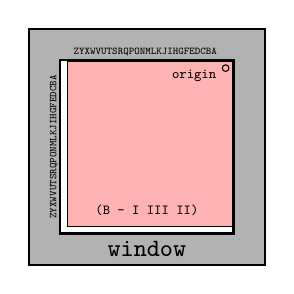
\begin{tikzpicture}
			% Table dimensions
			% Frame outer and inner sizes
			\pgfmathsetmacro{\frameOuter}{3}
			\pgfmathsetmacro{\frameInner}{2.2}
			\pgfmathsetmacro{\frameShift}{(\frameOuter - \frameInner)/2}

			% Position of the frame on the table (lower right corner, but centered)
			\pgfmathsetmacro{\fx}{2.5}
			\pgfmathsetmacro{\fy}{2.5}

			% Draw the picture frame outer square
			\fill[black!50!gray!40] (\fx, \fy) rectangle ({\fx +
					\frameOuter}, {\fy + \frameOuter});
			\fill[white] ({\fx + \frameShift}, {\fy + \frameShift})
			rectangle ({\fx + \frameOuter - \frameShift}, {\fy +
					\frameOuter - \frameShift});
			\draw[thick] (3, 3) rectangle (3+2.1, 3+2.08); % table edge
			\fill[red!30] (3, 3) rectangle (3+2.1, 3+2.08); % table edge

			% Optional outlines

			\draw[] (3+2,3+2.1-0.1) circle (1.2pt);

			\draw[thick] (\fx, \fy) rectangle ({\fx + \frameOuter}, {\fy +
					\frameOuter}); % frame outer
			\draw[thick] ({\fx + \frameShift}, {\fy + \frameShift})
			rectangle ({\fx + \frameOuter - \frameShift}, {\fy +
					\frameOuter - \frameShift}); % frame inner
			\node[font=\small, black] at ({\fx + \frameOuter/2}, {\fy +
				0.2}) {\texttt{window}};
			\node[font=\tiny, black] at ({\fx + \frameOuter/2}, {\fy + 0.2
				+ 0.5}) {\texttt{(B - I III II)}};
			\node[font=\tiny, black] at (3+2-0.4,3+2.1-0.2) {\texttt{origin}};
			\node[font=\tiny, ,scale=0.75, black] at (3+2-0.2-0.82,3+2.2)
			{\texttt{ZYXWVUTSRQPONMLKJIHGFEDCBA}};
			\node[font=\tiny, rotate=90,scale=0.75, black] at
			(3+2-1.36-0.82,3+2.2-1.2) {\texttt{ZYXWVUTSRQPONMLKJIHGFEDCBA}};
		\end{tikzpicture}
	}
	\caption{Sheet \texttt{(B - I III II)} shifted so that its origin
		is in location (\texttt{A}, \texttt{A}) in the window}
	\label{fig:shifted_sheet}
\end{figure}
\noindent We now consider our next indicator \texttt{AFQ} which
corresponds to sheet \texttt{(A - I III II)}. To align its origin we
place it in the window and translate it by(). After doing this, the
holes in both \texttt{(B - I III II)} and \texttt{(A - I III II)}
will only line up at specific locations leading to a window with
holes with light shining through as follow
\begin{figure}[H]
	\begin{center}
		\scalebox{0.5} {
			\begin{tabular}{c|cccccccccccccccccccccccccc}
				           & \texttt{Z} & \texttt{Y} & \texttt{X} & \texttt{W} &
				\texttt{V} & \texttt{U} & \texttt{T} & \texttt{S} &
				\texttt{R} & \texttt{Q} & \texttt{P} & \texttt{O} &
				\texttt{N} & \texttt{M} & \texttt{L} & \texttt{K} &
				\texttt{J} & \texttt{I} & \texttt{H} & \texttt{G} &
				\texttt{F} & \texttt{E} & \texttt{D} & \texttt{C} &
				\texttt{B} & \texttt{A}                                          \\ \hline
				\texttt{A} & \texttt{0} & \texttt{.} & \texttt{.} &
				\texttt{.} & \texttt{.} & \texttt{0} & \texttt{0} &
				\texttt{.} & \texttt{.} & \texttt{.} & \texttt{0} &
				\texttt{.} & \texttt{.} & \texttt{.} & \texttt{.} &
				\texttt{.} & \texttt{.} & \texttt{0} & \texttt{.} &
				\texttt{.} & \texttt{.} & \texttt{0} & \texttt{.} &
				\texttt{.} & \texttt{.} & \texttt{.}                             \\
				\texttt{B} & \texttt{.} & \texttt{.} & \texttt{.} &
				\texttt{.} & \texttt{.} & \texttt{.} & \texttt{.} &
				\texttt{0} & \texttt{0} & \texttt{0} & \texttt{.} &
				\texttt{.} & \texttt{.} & \texttt{.} & \texttt{.} &
				\texttt{.} & \texttt{.} & \texttt{.} & \texttt{.} &
				\texttt{.} & \texttt{.} & \texttt{.} & \texttt{.} &
				\texttt{.} & \texttt{.} & \texttt{.}                             \\
				\texttt{C} & \texttt{0} & \texttt{0} & \texttt{.} &
				\texttt{.} & \texttt{.} & \texttt{.} & \texttt{.} &
				\texttt{.} & \texttt{.} & \texttt{.} & \texttt{.} &
				\texttt{.} & \texttt{.} & \texttt{.} & \texttt{0} &
				\texttt{.} & \texttt{.} & \texttt{.} & \texttt{.} &
				\texttt{.} & \texttt{0} & \texttt{.} & \texttt{.} &
				\texttt{.} & \texttt{.} & \texttt{.}                             \\
				\texttt{D} & \texttt{.} & \texttt{.} & \texttt{.} &
				\texttt{.} & \texttt{.} & \texttt{.} & \texttt{.} &
				\texttt{.} & \texttt{0} & \texttt{.} & \texttt{.} &
				\texttt{.} & \texttt{0} & \texttt{.} & \texttt{.} &
				\texttt{.} & \texttt{.} & \texttt{.} & \texttt{.} &
				\texttt{0} & \texttt{.} & \texttt{.} & \texttt{.} &
				\texttt{0} & \texttt{0} & \texttt{.}                             \\
				\texttt{E} & \texttt{.} & \texttt{.} & \texttt{.} &
				\texttt{.} & \texttt{.} & \texttt{.} & \texttt{.} &
				\texttt{0} & \texttt{.} & \texttt{.} & \texttt{.} &
				\texttt{.} & \texttt{.} & \texttt{.} & \texttt{.} &
				\texttt{0} & \texttt{.} & \texttt{.} & \texttt{.} &
				\texttt{.} & \texttt{0} & \texttt{0} & \texttt{.} &
				\texttt{0} & \texttt{.} & \texttt{0}                             \\
				\texttt{F} & \texttt{.} & \texttt{.} & \texttt{.} &
				\texttt{.} & \texttt{.} & \texttt{0} & \texttt{0} &
				\texttt{.} & \texttt{0} & \texttt{.} & \texttt{0} &
				\texttt{.} & \texttt{0} & \texttt{0} & \texttt{.} &
				\texttt{0} & \texttt{.} & \texttt{.} & \texttt{.} &
				\texttt{.} & \texttt{0} & \texttt{.} & \texttt{.} &
				\texttt{.} & \texttt{.} & \texttt{.}                             \\
				\texttt{G} & \texttt{.} & \texttt{.} & \texttt{.} &
				\texttt{.} & \texttt{.} & \texttt{.} & \texttt{0} &
				\texttt{.} & \texttt{.} & \texttt{0} & \texttt{.} &
				\texttt{.} & \texttt{.} & \texttt{.} & \texttt{.} &
				\texttt{.} & \texttt{.} & \texttt{0} & \texttt{.} &
				\texttt{.} & \texttt{.} & \texttt{.} & \texttt{0} &
				\texttt{.} & \texttt{.} & \texttt{.}                             \\
				\texttt{H} & \texttt{.} & \texttt{0} & \texttt{.} &
				\texttt{.} & \texttt{0} & \texttt{.} & \texttt{0} &
				\texttt{.} & \texttt{0} & \texttt{.} & \texttt{.} &
				\texttt{.} & \texttt{.} & \texttt{0} & \texttt{.} &
				\texttt{0} & \texttt{.} & \texttt{.} & \texttt{0} &
				\texttt{.} & \texttt{.} & \texttt{.} & \texttt{.} &
				\texttt{.} & \texttt{.} & \texttt{.}                             \\
				\texttt{I} & \texttt{.} & \texttt{.} & \texttt{.} &
				\texttt{.} & \texttt{.} & \texttt{.} & \texttt{.} &
				\texttt{.} & \texttt{0} & \texttt{0} & \texttt{.} &
				\texttt{.} & \texttt{0} & \texttt{.} & \texttt{.} &
				\texttt{0} & \texttt{.} & \texttt{.} & \texttt{.} &
				\texttt{0} & \texttt{.} & \texttt{.} & \texttt{.} &
				\texttt{.} & \texttt{.} & \texttt{.}                             \\
				\texttt{J} & \texttt{.} & \texttt{.} & \texttt{.} &
				\texttt{.} & \texttt{.} & \texttt{.} & \texttt{.} &
				\texttt{.} & \texttt{.} & \texttt{.} & \texttt{.} &
				\texttt{.} & \texttt{.} & \texttt{.} & \texttt{.} &
				\texttt{.} & \texttt{.} & \texttt{.} & \texttt{.} &
				\texttt{.} & \texttt{.} & \texttt{0} & \texttt{.} &
				\texttt{.} & \texttt{.} & \texttt{.}                             \\
				\texttt{K} & \texttt{.} & \texttt{.} & \texttt{.} &
				\texttt{.} & \texttt{.} & \texttt{.} & \texttt{.} &
				\texttt{0} & \texttt{.} & \texttt{.} & \texttt{.} &
				\texttt{.} & \texttt{.} & \texttt{.} & \texttt{.} &
				\texttt{.} & \texttt{0} & \texttt{.} & \texttt{0} &
				\texttt{.} & \texttt{.} & \texttt{.} & \texttt{.} &
				\texttt{.} & \texttt{.} & \texttt{.}                             \\
				\texttt{L} & \texttt{.} & \texttt{.} & \texttt{.} &
				\texttt{0} & \texttt{.} & \texttt{.} & \texttt{.} &
				\texttt{.} & \texttt{.} & \texttt{.} & \texttt{0} &
				\texttt{.} & \texttt{0} & \texttt{.} & \texttt{.} &
				\texttt{.} & \texttt{.} & \texttt{.} & \texttt{0} &
				\texttt{.} & \texttt{.} & \texttt{.} & \texttt{.} &
				\texttt{.} & \texttt{.} & \texttt{.}                             \\
				\texttt{M} & \texttt{0} & \texttt{0} & \texttt{.} &
				\texttt{0} & \texttt{0} & \texttt{.} & \texttt{0} &
				\texttt{.} & \texttt{.} & \texttt{.} & \texttt{0} &
				\texttt{.} & \texttt{.} & \texttt{0} & \texttt{0} &
				\texttt{.} & \texttt{.} & \texttt{.} & \texttt{0} &
				\texttt{.} & \texttt{.} & \texttt{.} & \texttt{.} &
				\texttt{.} & \texttt{.} & \texttt{.}                             \\
				\texttt{N} & \texttt{.} & \texttt{.} & \texttt{.} &
				\texttt{.} & \texttt{.} & \texttt{.} & \texttt{.} &
				\texttt{.} & \texttt{0} & \texttt{.} & \texttt{.} &
				\texttt{.} & \texttt{.} & \texttt{0} & \texttt{.} &
				\texttt{.} & \texttt{.} & \texttt{.} & \texttt{.} &
				\texttt{0} & \texttt{.} & \texttt{.} & \texttt{.} &
				\texttt{.} & \texttt{.} & \texttt{.}                             \\
				\texttt{O} & \texttt{.} & \texttt{.} & \texttt{.} &
				\texttt{0} & \texttt{.} & \texttt{.} & \texttt{.} &
				\texttt{.} & \texttt{.} & \texttt{.} & \texttt{.} &
				\texttt{.} & \texttt{.} & \texttt{.} & \texttt{.} &
				\texttt{0} & \texttt{.} & \texttt{.} & \texttt{.} &
				\texttt{0} & \texttt{.} & \texttt{.} & \texttt{0} &
				\texttt{0} & \texttt{.} & \texttt{.}                             \\
				\texttt{P} & \texttt{.} & \texttt{.} & \texttt{.} &
				\texttt{.} & \texttt{0} & \texttt{.} & \texttt{0} &
				\texttt{.} & \texttt{.} & \texttt{.} & \texttt{0} &
				\texttt{.} & \texttt{.} & \texttt{.} & \texttt{.} &
				\texttt{0} & \texttt{0} & \texttt{.} & \texttt{.} &
				\texttt{.} & \texttt{.} & \texttt{.} & \texttt{.} &
				\texttt{.} & \texttt{.} & \texttt{0}                             \\
				\texttt{Q} & \texttt{.} & \texttt{.} & \texttt{.} &
				\texttt{.} & \texttt{.} & \texttt{.} & \texttt{.} &
				\texttt{.} & \texttt{.} & \texttt{0} & \texttt{.} &
				\texttt{.} & \texttt{.} & \texttt{.} & \texttt{.} &
				\texttt{.} & \texttt{0} & \texttt{0} & \texttt{.} &
				\texttt{.} & \texttt{.} & \texttt{.} & \texttt{.} &
				\texttt{.} & \texttt{.} & \texttt{.}                             \\
				\texttt{R} & \texttt{.} & \texttt{0} & \texttt{.} &
				\texttt{.} & \texttt{.} & \texttt{.} & \texttt{.} &
				\texttt{.} & \texttt{.} & \texttt{.} & \texttt{0} &
				\texttt{.} & \texttt{.} & \texttt{.} & \texttt{.} &
				\texttt{.} & \texttt{0} & \texttt{.} & \texttt{0} &
				\texttt{.} & \texttt{.} & \texttt{.} & \texttt{.} &
				\texttt{.} & \texttt{0} & \texttt{.}                             \\
				\texttt{S} & \texttt{0} & \texttt{.} & \texttt{.} &
				\texttt{.} & \texttt{.} & \texttt{.} & \texttt{.} &
				\texttt{0} & \texttt{0} & \texttt{.} & \texttt{.} &
				\texttt{.} & \texttt{.} & \texttt{.} & \texttt{.} &
				\texttt{.} & \texttt{.} & \texttt{0} & \texttt{.} &
				\texttt{.} & \texttt{0} & \texttt{.} & \texttt{.} &
				\texttt{.} & \texttt{.} & \texttt{.}                             \\
				\texttt{T} & \texttt{.} & \texttt{0} & \texttt{0} &
				\texttt{0} & \texttt{.} & \texttt{0} & \texttt{.} &
				\texttt{.} & \texttt{.} & \texttt{.} & \texttt{0} &
				\texttt{0} & \texttt{0} & \texttt{.} & \texttt{.} &
				\texttt{.} & \texttt{.} & \texttt{.} & \texttt{.} &
				\texttt{.} & \texttt{0} & \texttt{.} & \texttt{.} &
				\texttt{0} & \texttt{.} & \texttt{.}                             \\
				\texttt{U} & \texttt{.} & \texttt{.} & \texttt{.} &
				\texttt{.} & \texttt{0} & \texttt{.} & \texttt{.} &
				\texttt{.} & \texttt{0} & \texttt{.} & \texttt{0} &
				\texttt{.} & \texttt{0} & \texttt{.} & \texttt{.} &
				\texttt{.} & \texttt{.} & \texttt{.} & \texttt{.} &
				\texttt{.} & \texttt{.} & \texttt{.} & \texttt{.} &
				\texttt{0} & \texttt{.} & \texttt{.}                             \\
				\texttt{V} & \texttt{0} & \texttt{.} & \texttt{.} &
				\texttt{.} & \texttt{.} & \texttt{.} & \texttt{.} &
				\texttt{.} & \texttt{.} & \texttt{.} & \texttt{.} &
				\texttt{0} & \texttt{0} & \texttt{.} & \texttt{.} &
				\texttt{.} & \texttt{.} & \texttt{.} & \texttt{.} &
				\texttt{.} & \texttt{.} & \texttt{0} & \texttt{.} &
				\texttt{0} & \texttt{.} & \texttt{.}                             \\
				\texttt{W} & \texttt{.} & \texttt{.} & \texttt{.} &
				\texttt{.} & \texttt{0} & \texttt{.} & \texttt{.} &
				\texttt{.} & \texttt{.} & \texttt{.} & \texttt{.} &
				\texttt{.} & \texttt{.} & \texttt{.} & \texttt{.} &
				\texttt{0} & \texttt{.} & \texttt{.} & \texttt{.} &
				\texttt{0} & \texttt{.} & \texttt{.} & \texttt{0} &
				\texttt{0} & \texttt{.} & \texttt{.}                             \\
				\texttt{X} & \texttt{.} & \texttt{0} & \texttt{0} &
				\texttt{.} & \texttt{.} & \texttt{.} & \texttt{.} &
				\texttt{.} & \texttt{.} & \texttt{.} & \texttt{0} &
				\texttt{0} & \texttt{.} & \texttt{.} & \texttt{.} &
				\texttt{.} & \texttt{0} & \texttt{.} & \texttt{0} &
				\texttt{0} & \texttt{.} & \texttt{0} & \texttt{.} &
				\texttt{.} & \texttt{.} & \texttt{0}                             \\
				\texttt{Y} & \texttt{.} & \texttt{.} & \texttt{0} &
				\texttt{.} & \texttt{.} & \texttt{0} & \texttt{.} &
				\texttt{.} & \texttt{.} & \texttt{.} & \texttt{.} &
				\texttt{.} & \texttt{.} & \texttt{.} & \texttt{.} &
				\texttt{.} & \texttt{.} & \texttt{.} & \texttt{.} &
				\texttt{0} & \texttt{.} & \texttt{.} & \texttt{0} &
				\texttt{.} & \texttt{.} & \texttt{.}                             \\
				\texttt{Z} & \texttt{.} & \texttt{0} & \texttt{.} &
				\texttt{.} & \texttt{.} & \texttt{.} & \texttt{.} &
				\texttt{.} & \texttt{.} & \texttt{.} & \texttt{.} &
				\texttt{.} & \texttt{.} & \texttt{.} & \texttt{.} &
				\texttt{.} & \texttt{.} & \texttt{0} & \texttt{.} &
				\texttt{0} & \texttt{.} & \texttt{.} & \texttt{.} &
				\texttt{.} & \texttt{.} & \texttt{.}                             \\
			\end{tabular}
		}
	\end{center}
	\caption{Window after lining up sheets for the first two indicators
		\texttt{BWY} and \texttt{AFQ}}
\end{figure}
\noindent Continuing in this fashion, placing each the origin of each
sheet corresponding to an indicator in the top right of our window,
we are left with the following window

\begin{figure}[H]
	\begin{center}
		\scalebox{0.5}{
			\begin{tabular}{c|cccccccccccccccccccccccccc}
				           & \texttt{Z} & \texttt{Y} & \texttt{X} & \texttt{W} &
				\texttt{V} & \texttt{U} & \texttt{T} & \texttt{S} &
				\texttt{R} & \texttt{Q} & \texttt{P} & \texttt{O} &
				\texttt{N} & \texttt{M} & \texttt{L} & \texttt{K} &
				\texttt{J} & \texttt{I} & \texttt{H} & \texttt{G} &
				\texttt{F} & \texttt{E} & \texttt{D} & \texttt{C} &
				\texttt{B} & \texttt{A}                                          \\ \hline
				\texttt{A} & \texttt{.} & \texttt{.} & \texttt{.} &
				\texttt{.} & \texttt{.} & \texttt{.} & \texttt{.} &
				\texttt{.} & \texttt{.} & \texttt{.} & \texttt{.} &
				\texttt{.} & \texttt{.} & \texttt{.} & \texttt{.} &
				\texttt{.} & \texttt{.} & \texttt{.} & \texttt{.} &
				\texttt{.} & \texttt{.} & \texttt{.} & \texttt{.} &
				\texttt{.} & \texttt{.} & \texttt{.}                             \\
				\texttt{B} & \texttt{.} & \texttt{.} & \texttt{.} &
				\texttt{.} & \texttt{.} & \texttt{.} & \texttt{.} &
				\texttt{.} & \texttt{.} & \texttt{.} & \texttt{.} &
				\texttt{.} & \texttt{.} & \texttt{.} & \texttt{.} &
				\texttt{.} & \texttt{.} & \texttt{.} & \texttt{.} &
				\texttt{.} & \texttt{.} & \texttt{.} & \texttt{.} &
				\texttt{.} & \texttt{.} & \texttt{.}                             \\
				\texttt{C} & \texttt{.} & \texttt{.} & \texttt{.} &
				\texttt{.} & \texttt{.} & \texttt{.} & \texttt{.} &
				\texttt{.} & \texttt{.} & \texttt{.} & \texttt{.} &
				\texttt{.} & \texttt{.} & \texttt{.} & \texttt{.} &
				\texttt{.} & \texttt{.} & \texttt{.} & \texttt{.} &
				\texttt{.} & \texttt{.} & \texttt{.} & \texttt{.} &
				\texttt{.} & \texttt{.} & \texttt{.}                             \\
				\texttt{D} & \texttt{.} & \texttt{.} & \texttt{.} &
				\texttt{.} & \texttt{.} & \texttt{.} & \texttt{.} &
				\texttt{.} & \texttt{.} & \texttt{.} & \texttt{.} &
				\texttt{.} & \texttt{.} & \texttt{.} & \texttt{.} &
				\texttt{.} & \texttt{.} & \texttt{.} & \texttt{.} &
				\texttt{.} & \texttt{.} & \texttt{.} & \texttt{.} &
				\texttt{.} & \texttt{.} & \texttt{.}                             \\
				\texttt{E} & \texttt{.} & \texttt{.} & \texttt{.} &
				\texttt{.} & \texttt{.} & \texttt{.} & \texttt{.} &
				\texttt{.} & \texttt{.} & \texttt{.} & \texttt{.} &
				\texttt{.} & \texttt{.} & \texttt{.} & \texttt{.} &
				\texttt{.} & \texttt{.} & \texttt{.} & \texttt{.} &
				\texttt{.} & \texttt{.} & \texttt{.} & \texttt{.} &
				\texttt{.} & \texttt{.} & \texttt{.}                             \\
				\texttt{F} & \texttt{.} & \texttt{.} & \texttt{.} &
				\texttt{.} & \texttt{.} & \texttt{.} & \texttt{.} &
				\texttt{.} & \texttt{.} & \texttt{.} & \texttt{.} &
				\texttt{.} & \texttt{.} & \texttt{.} & \texttt{.} &
				\texttt{.} & \texttt{.} & \texttt{.} & \texttt{.} &
				\texttt{.} & \texttt{.} & \texttt{.} & \texttt{.} &
				\texttt{.} & \texttt{.} & \texttt{.}                             \\
				\texttt{G} & \texttt{.} & \texttt{.} & \texttt{.} &
				\texttt{.} & \texttt{.} & \texttt{.} & \texttt{.} &
				\texttt{.} & \texttt{.} & \texttt{.} & \texttt{.} &
				\texttt{.} & \texttt{.} & \texttt{.} & \texttt{.} &
				\texttt{.} & \texttt{.} & \texttt{.} & \texttt{.} &
				\texttt{.} & \texttt{.} & \texttt{.} & \texttt{.} &
				\texttt{.} & \texttt{.} & \texttt{.}                             \\
				\texttt{H} & \texttt{.} & \texttt{.} & \texttt{.} &
				\texttt{.} & \texttt{.} & \texttt{.} & \texttt{.} &
				\texttt{.} & \texttt{.} & \texttt{.} & \texttt{.} &
				\texttt{.} & \texttt{.} & \texttt{.} & \texttt{.} &
				\texttt{.} & \texttt{.} & \texttt{.} & \texttt{.} &
				\texttt{.} & \texttt{.} & \texttt{.} & \texttt{.} &
				\texttt{.} & \texttt{.} & \texttt{.}                             \\
				\texttt{I} & \texttt{.} & \texttt{.} & \texttt{.} &
				\texttt{.} & \texttt{.} & \texttt{.} & \texttt{.} &
				\texttt{.} & \texttt{.} & \texttt{.} & \texttt{.} &
				\texttt{.} & \texttt{.} & \texttt{.} & \texttt{.} &
				\texttt{.} & \texttt{.} & \texttt{.} & \texttt{.} &
				\texttt{.} & \texttt{.} & \texttt{.} & \texttt{.} &
				\texttt{.} & \texttt{.} & \texttt{.}                             \\
				\texttt{J} & \texttt{.} & \texttt{.} & \texttt{.} &
				\texttt{.} & \texttt{.} & \texttt{.} & \texttt{.} &
				\texttt{.} & \texttt{.} & \texttt{.} & \texttt{.} &
				\texttt{.} & \texttt{.} & \texttt{.} & \texttt{.} &
				\texttt{.} & \texttt{.} & \texttt{.} & \texttt{.} &
				\texttt{.} & \texttt{.} & \texttt{.} & \texttt{.} &
				\texttt{.} & \texttt{.} & \texttt{.}                             \\
				\texttt{K} & \texttt{.} & \texttt{.} & \texttt{.} &
				\texttt{.} & \texttt{.} & \texttt{.} & \texttt{.} &
				\texttt{.} & \texttt{.} & \texttt{.} & \texttt{.} &
				\texttt{.} & \texttt{.} & \texttt{.} & \texttt{.} &
				\texttt{.} & \texttt{.} & \texttt{.} & \texttt{.} &
				\texttt{.} & \texttt{.} & \texttt{.} & \texttt{.} &
				\texttt{.} & \texttt{.} & \texttt{.}                             \\
				\texttt{L} & \texttt{.} & \texttt{.} & \texttt{.} &
				\texttt{.} & \texttt{.} & \texttt{.} & \texttt{.} &
				\texttt{.} & \texttt{.} & \texttt{.} & \texttt{.} &
				\texttt{.} & \texttt{.} & \texttt{.} & \texttt{.} &
				\texttt{.} & \texttt{.} & \texttt{.} & \texttt{.} &
				\texttt{.} & \texttt{.} & \texttt{.} & \texttt{.} &
				\texttt{.} & \texttt{.} & \texttt{.}                             \\
				\texttt{M} & \texttt{.} & \texttt{.} & \texttt{.} &
				\texttt{.} & \texttt{.} & \texttt{.} & \texttt{.} &
				\texttt{.} & \texttt{.} & \texttt{.} & \texttt{.} &
				\texttt{.} & \texttt{.} & \texttt{.} & \texttt{.} &
				\texttt{.} & \texttt{.} & \texttt{.} & \texttt{.} &
				\texttt{.} & \texttt{.} & \texttt{.} & \texttt{.} &
				\texttt{.} & \texttt{.} & \texttt{.}                             \\
				\texttt{N} & \texttt{.} & \texttt{.} & \texttt{.} &
				\texttt{.} & \texttt{.} & \texttt{.} & \texttt{.} &
				\texttt{.} & \texttt{.} & \texttt{.} & \texttt{.} &
				\texttt{.} & \texttt{.} & \texttt{.} & \texttt{.} &
				\texttt{.} & \texttt{.} & \texttt{.} & \texttt{.} &
				\texttt{.} & \texttt{.} & \texttt{.} & \texttt{.} &
				\texttt{.} & \texttt{.} & \texttt{.}                             \\
				\texttt{O} & \texttt{.} & \texttt{.} & \texttt{.} &
				\texttt{.} & \texttt{.} & \texttt{.} & \texttt{.} &
				\texttt{.} & \texttt{.} & \texttt{.} & \texttt{.} &
				\texttt{.} & \texttt{.} & \texttt{.} & \texttt{.} &
				\texttt{.} & \texttt{.} & \texttt{.} & \texttt{.} &
				\texttt{.} & \texttt{.} & \texttt{.} & \texttt{.} &
				\texttt{.} & \texttt{.} & \texttt{.}                             \\
				\texttt{P} & \texttt{.} & \texttt{.} & \texttt{.} &
				\texttt{.} & \texttt{.} & \texttt{.} & \texttt{.} &
				\texttt{.} & \texttt{.} & \texttt{.} & \texttt{.} &
				\texttt{.} & \texttt{.} & \texttt{.} & \texttt{.} &
				\texttt{.} & \texttt{.} & \texttt{.} & \texttt{.} &
				\texttt{.} & \texttt{.} & \texttt{.} & \texttt{.} &
				\texttt{.} & \texttt{.} & \texttt{.}                             \\
				\texttt{Q} & \texttt{.} & \texttt{.} & \texttt{.} &
				\texttt{.} & \texttt{.} & \texttt{.} & \texttt{.} &
				\texttt{.} & \texttt{.} & \texttt{.} & \texttt{.} &
				\texttt{.} & \texttt{.} & \texttt{.} & \texttt{.} &
				\texttt{.} & \texttt{.} & \texttt{.} & \texttt{.} &
				\texttt{.} & \texttt{.} & \texttt{.} & \texttt{.} &
				\texttt{.} & \texttt{.} & \texttt{.}                             \\
				\texttt{R} & \texttt{.} & \texttt{.} & \texttt{.} &
				\texttt{.} & \texttt{.} & \texttt{.} & \texttt{.} &
				\texttt{.} & \texttt{.} & \texttt{.} & \texttt{.} &
				\texttt{.} & \texttt{.} & \texttt{.} & \texttt{.} &
				\texttt{.} & \texttt{.} & \texttt{.} & \texttt{.} &
				\texttt{.} & \texttt{.} & \texttt{.} & \texttt{.} &
				\texttt{.} & \texttt{.} & \texttt{.}                             \\
				\texttt{S} & \texttt{.} & \texttt{.} & \texttt{.} &
				\texttt{.} & \texttt{.} & \texttt{.} & \texttt{.} &
				\texttt{.} & \texttt{.} & \texttt{.} & \texttt{.} &
				\texttt{.} & \texttt{.} & \texttt{.} & \texttt{.} &
				\texttt{.} & \texttt{.} & \texttt{.} & \texttt{.} &
				\texttt{.} & \texttt{.} & \texttt{.} & \texttt{.} &
				\texttt{.} & \texttt{.} & \texttt{.}                             \\
				\texttt{T} & \texttt{.} & \texttt{.} & \texttt{.} &
				\texttt{.} & \texttt{.} & \texttt{.} & \texttt{.} &
				\texttt{.} & \texttt{.} & \texttt{.} & \texttt{.} &
				\texttt{.} & \texttt{.} & \texttt{.} & \texttt{.} &
				\texttt{.} & \texttt{.} & \texttt{.} & \texttt{.} &
				\texttt{.} & \texttt{.} & \texttt{.} & \texttt{.} &
				\texttt{.} & \texttt{.} & \texttt{.}                             \\
				\texttt{U} & \texttt{.} & \texttt{.} & \texttt{.} &
				\texttt{.} & \texttt{.} & \texttt{.} & \texttt{.} &
				\texttt{.} & \texttt{.} & \texttt{.} & \texttt{.} &
				\texttt{.} & \texttt{.} & \texttt{.} & \texttt{.} &
				\texttt{.} & \texttt{.} & \texttt{.} & \texttt{.} &
				\texttt{.} & \texttt{.} & \texttt{.} & \texttt{.} &
				\texttt{.} & \texttt{.} & \texttt{.}                             \\
				\texttt{V} & \texttt{.} & \texttt{.} & \texttt{.} &
				\texttt{.} & \texttt{.} & \texttt{.} & \texttt{.} &
				\texttt{.} & \texttt{.} & \texttt{.} & \texttt{.} &
				\texttt{.} & \texttt{.} & \texttt{.} & \texttt{.} &
				\texttt{.} & \texttt{.} & \texttt{.} & \texttt{.} &
				\texttt{.} & \texttt{.} & \texttt{.} & \texttt{.} &
				\texttt{.} & \texttt{.} & \texttt{.}                             \\
				\texttt{W} & \texttt{.} & \texttt{.} & \texttt{.} &
				\texttt{.} & \texttt{.} & \texttt{.} & \texttt{.} &
				\texttt{.} & \texttt{.} & \texttt{.} & \texttt{.} &
				\texttt{.} & \texttt{.} & \texttt{.} & \texttt{.} &
				\texttt{.} & \texttt{.} & \texttt{.} & \texttt{.} &
				\texttt{.} & \texttt{.} & \texttt{.} & \texttt{.} &
				\texttt{.} & \texttt{.} & \texttt{.}                             \\
				\texttt{X} & \texttt{.} & \texttt{.} & \texttt{.} &
				\texttt{.} & \texttt{.} & \texttt{.} & \texttt{.} &
				\texttt{.} & \texttt{.} & \texttt{.} & \texttt{.} &
				\texttt{.} & \texttt{.} & \texttt{.} & \texttt{.} &
				\texttt{.} & \texttt{.} & \texttt{.} & \texttt{.} &
				\texttt{.} & \texttt{.} & \texttt{.} & \texttt{.} &
				\texttt{.} & \texttt{.} & \texttt{.}                             \\
				\texttt{Y} & \texttt{.} & \texttt{.} & \texttt{.} &
				\texttt{.} & \texttt{.} & \texttt{.} & \texttt{.} &
				\texttt{.} & \texttt{.} & \texttt{.} & \texttt{.} &
				\texttt{.} & \texttt{.} & \texttt{.} & \texttt{.} &
				\texttt{.} & \texttt{.} & \texttt{.} & \texttt{.} &
				\texttt{.} & \texttt{.} & \texttt{.} & \texttt{.} &
				\texttt{.} & \texttt{.} & \texttt{.}                             \\
				\texttt{Z} & \texttt{.} & \texttt{.} & \texttt{.} &
				\texttt{.} & \texttt{.} & \texttt{.} & \texttt{.} &
				\texttt{.} & \texttt{.} & \texttt{.} & \texttt{.} &
				\texttt{.} & \texttt{.} & \texttt{.} & \texttt{.} &
				\texttt{.} & \texttt{.} & \texttt{.} & \texttt{.} &
				\texttt{.} & \texttt{.} & \texttt{.} & \texttt{.} &
				\texttt{.} & \texttt{.} & \texttt{.}                             \\
			\end{tabular}
		}
	\end{center}
	\caption{Window setting after overlaying sheets corresponding to
		all indicators}
\end{figure}
\noindent That is, all holes are blocked and thus there is no
position for which the rotors \texttt{I III II} and ring settings
beginning with \texttt{A} can generate the observed females.
\\\\This only tested all ring settings beginning with \texttt{A}. To
test the ring settings beginning with \texttt{B} we can move each
sheet letter back by $1$. That is, instead of sheet \texttt{(B - I
	III II)} use sheet \texttt{(A - I III II)}, and peform the exact same
procedure. Iterating in this fashion through each possible letter in
the leftmost ring setting, we will find some sheets which do have
light peering through holes in all the sheets. Many of these
settings, after testing, will be ruled out. However, eventually when
we have moved the letter on each sheet back $3$ times, which
corresponds to the leftmost ring settting being \texttt{D}, we will
see the following window
\begin{figure}[H]
	\begin{center}
		\scalebox{0.5} {
			\begin{tabular}{c|cccccccccccccccccccccccccc}
				           & \texttt{Z} & \texttt{Y} & \texttt{X} & \texttt{W} &
				\texttt{V} & \texttt{U} & \texttt{T} & \texttt{S} &
				\texttt{R} & \texttt{Q} & \texttt{P} & \texttt{O} &
				\texttt{N} & \texttt{M} & \texttt{L} & \texttt{K} &
				\texttt{J} & \texttt{I} & \texttt{H} & \texttt{G} &
				\texttt{F} & \texttt{E} & \texttt{D} & \texttt{C} &
				\texttt{B} & \texttt{A}                                          \\ \hline
				\texttt{A} & \texttt{.} & \texttt{.} & \texttt{.} &
				\texttt{.} & \texttt{.} & \texttt{.} & \texttt{.} &
				\texttt{.} & \texttt{.} & \texttt{.} & \texttt{.} &
				\texttt{.} & \texttt{.} & \texttt{.} & \texttt{.} &
				\texttt{.} & \texttt{.} & \texttt{.} & \texttt{.} &
				\texttt{.} & \texttt{.} & \texttt{.} & \texttt{.} &
				\texttt{.} & \texttt{.} & \texttt{.}                             \\
				\texttt{B} & \texttt{.} & \texttt{.} & \texttt{.} &
				\texttt{.} & \texttt{.} & \texttt{.} & \texttt{.} &
				\texttt{.} & \texttt{.} & \texttt{.} & \texttt{.} &
				\texttt{.} & \texttt{.} & \texttt{.} & \texttt{.} &
				\texttt{.} & \texttt{.} & \texttt{.} & \texttt{.} &
				\texttt{.} & \texttt{.} & \texttt{.} & \texttt{.} &
				\texttt{.} & \texttt{.} & \texttt{.}                             \\
				\texttt{C} & \texttt{.} & \texttt{.} & \texttt{.} &
				\texttt{.} & \texttt{.} & \texttt{.} & \texttt{.} &
				\texttt{.} & \texttt{.} & \texttt{.} & \texttt{.} &
				\texttt{.} & \texttt{.} & \texttt{.} & \texttt{.} &
				\texttt{.} & \texttt{.} & \texttt{.} & \texttt{.} &
				\texttt{.} & \texttt{.} & \texttt{.} & \texttt{.} &
				\texttt{.} & \texttt{.} & \texttt{.}                             \\
				\texttt{D} & \texttt{.} & \texttt{.} & \texttt{.} &
				\texttt{.} & \texttt{.} & \texttt{.} & \texttt{.} &
				\texttt{.} & \texttt{.} & \texttt{.} & \texttt{.} &
				\texttt{.} & \texttt{.} & \texttt{.} & \texttt{.} &
				\texttt{.} & \texttt{.} & \texttt{.} & \texttt{.} &
				\texttt{.} & \texttt{.} & \texttt{.} & \texttt{.} &
				\texttt{.} & \texttt{.} & \texttt{.}                             \\
				\texttt{E} & \texttt{.} & \texttt{.} & \texttt{.} &
				\texttt{.} & \texttt{.} & \texttt{.} & \texttt{.} &
				\texttt{.} & \texttt{.} & \texttt{.} & \texttt{.} &
				\texttt{.} & \texttt{.} & \texttt{.} & \texttt{.} &
				\texttt{.} & \texttt{.} & \texttt{.} & \texttt{.} &
				\texttt{.} & \texttt{.} & \texttt{.} & \texttt{.} &
				\texttt{.} & \texttt{.} & \texttt{.}                             \\
				\texttt{F} & \texttt{.} & \texttt{.} & \texttt{.} &
				\texttt{.} & \texttt{.} & \texttt{.} & \texttt{.} &
				\texttt{.} & \texttt{.} & \texttt{.} & \texttt{.} &
				\texttt{.} & \texttt{.} & \texttt{.} & \texttt{.} &
				\texttt{.} & \texttt{.} & \texttt{.} & \texttt{.} &
				\texttt{.} & \texttt{.} & \texttt{.} & \texttt{.} &
				\texttt{.} & \texttt{.} & \texttt{.}                             \\
				\texttt{G} & \texttt{.} & \texttt{.} & \texttt{.} &
				\texttt{.} & \texttt{.} & \texttt{.} & \texttt{.} &
				\texttt{.} & \texttt{.} & \texttt{.} & \texttt{.} &
				\texttt{.} & \texttt{.} & \texttt{.} & \texttt{.} &
				\texttt{.} & \texttt{.} & \texttt{.} & \texttt{.} &
				\texttt{.} & \texttt{.} & \texttt{.} & \texttt{.} &
				\texttt{.} & \texttt{.} & \texttt{.}                             \\
				\texttt{H} & \texttt{.} & \texttt{.} & \texttt{.} &
				\texttt{.} & \texttt{.} & \texttt{.} & \texttt{.} &
				\texttt{.} & \texttt{.} & \texttt{.} & \texttt{.} &
				\texttt{.} & \texttt{.} & \texttt{.} & \texttt{.} &
				\texttt{.} & \texttt{.} & \texttt{.} & \texttt{.} &
				\texttt{.} & \texttt{.} & \texttt{.} & \texttt{.} &
				\texttt{.} & \texttt{.} & \texttt{.}                             \\
				\texttt{I} & \texttt{.} & \texttt{.} & \texttt{.} &
				\texttt{.} & \texttt{.} & \texttt{.} & \texttt{.} &
				\texttt{.} & \texttt{.} & \texttt{.} & \texttt{.} &
				\texttt{.} & \texttt{.} & \texttt{.} & \texttt{.} &
				\texttt{.} & \texttt{.} & \texttt{.} & \texttt{.} &
				\texttt{.} & \texttt{.} & \texttt{.} & \texttt{.} &
				\texttt{.} & \texttt{.} & \texttt{.}                             \\
				\texttt{J} & \texttt{.} & \texttt{.} & \texttt{.} &
				\texttt{.} & \texttt{.} & \texttt{.} & \texttt{.} &
				\texttt{.} & \texttt{.} & \texttt{.} & \texttt{.} &
				\texttt{.} & \texttt{.} & \texttt{.} & \texttt{.} &
				\texttt{.} & \texttt{.} & \texttt{.} & \texttt{.} &
				\texttt{.} & \texttt{.} & \texttt{.} & \texttt{.} &
				\texttt{.} & \texttt{.} & \texttt{.}                             \\
				\texttt{K} & \texttt{.} & \texttt{.} & \texttt{.} &
				\texttt{.} & \texttt{.} & \texttt{.} & \texttt{.} &
				\texttt{.} & \texttt{.} & \texttt{.} & \texttt{.} &
				\texttt{.} & \texttt{.} & \texttt{.} & \texttt{.} &
				\texttt{.} & \texttt{.} & \texttt{.} & \texttt{.} &
				\texttt{.} & \texttt{.} & \texttt{.} & \texttt{.} &
				\texttt{.} & \texttt{.} & \texttt{.}                             \\
				\texttt{L} & \texttt{.} & \texttt{.} & \texttt{.} &
				\texttt{.} & \texttt{.} & \texttt{.} & \texttt{.} &
				\texttt{.} & \texttt{.} & \texttt{.} & \texttt{.} &
				\texttt{.} & \texttt{.} & \texttt{.} & \texttt{.} &
				\texttt{.} & \texttt{.} & \texttt{.} & \texttt{.} &
				\texttt{.} & \texttt{.} & \texttt{.} & \texttt{.} &
				\texttt{.} & \texttt{.} & \texttt{.}                             \\
				\texttt{M} & \texttt{.} & \texttt{.} & \texttt{.} &
				\texttt{.} & \texttt{.} & \texttt{.} & \texttt{.} &
				\texttt{.} & \texttt{.} & \texttt{.} & \texttt{.} &
				\texttt{.} & \texttt{.} & \texttt{.} & \texttt{.} &
				\texttt{.} & \texttt{.} & \texttt{.} & \texttt{.} &
				\texttt{.} & \texttt{.} & \texttt{.} & \texttt{.} &
				\texttt{.} & \texttt{.} & \texttt{.}                             \\
				\texttt{N} & \texttt{.} & \texttt{.} & \texttt{.} &
				\texttt{.} & \texttt{.} & \texttt{.} & \texttt{.} &
				\texttt{.} & \texttt{.} & \texttt{.} & \texttt{.} &
				\texttt{.} & \texttt{.} & \texttt{.} & \texttt{.} &
				\texttt{.} & \texttt{.} & \texttt{.} & \texttt{.} &
				\texttt{.} & \texttt{.} & \texttt{.} & \texttt{.} &
				\texttt{.} & \texttt{.} & \texttt{.}                             \\
				\texttt{O} & \texttt{.} & \texttt{.} & \texttt{.} &
				\texttt{.} & \texttt{.} & \texttt{.} & \texttt{.} &
				\texttt{.} & \texttt{.} & \texttt{.} & \texttt{.} &
				\texttt{.} & \texttt{.} & \texttt{.} & \texttt{.} &
				\texttt{.} & \texttt{.} & \texttt{.} & \texttt{.} &
				\texttt{.} & \texttt{.} & \texttt{.} & \texttt{.} &
				\texttt{.} & \texttt{.} & \texttt{.}                             \\
				\texttt{P} & \texttt{.} & \texttt{.} & \texttt{.} &
				\texttt{.} & \texttt{.} & \texttt{.} & \texttt{.} &
				\texttt{.} & \texttt{.} & \texttt{.} & \texttt{.} &
				\texttt{.} & \texttt{.} & \texttt{.} & \texttt{.} &
				\texttt{.} & \texttt{.} & \texttt{.} & \texttt{.} &
				\texttt{.} & \texttt{.} & \texttt{.} & \texttt{.} &
				\texttt{.} & \texttt{.} & \texttt{.}                             \\
				\texttt{Q} & \texttt{.} & \texttt{.} & \texttt{.} &
				\texttt{.} & \texttt{.} & \texttt{.} & \texttt{.} &
				\texttt{.} & \texttt{.} & \texttt{.} & \texttt{.} &
				\texttt{.} & \texttt{.} & \texttt{.} & \texttt{.} &
				\texttt{.} & \texttt{.} & \texttt{.} & \texttt{.} &
				\texttt{.} & \texttt{.} & \texttt{.} & \texttt{.} &
				\texttt{.} & \texttt{.} & \texttt{.}                             \\
				\texttt{R} & \texttt{.} & \texttt{.} & \texttt{.} &
				\texttt{.} & \texttt{.} & \texttt{.} & \texttt{.} &
				\texttt{.} & \texttt{.} & \texttt{.} & \texttt{.} &
				\texttt{.} & \texttt{.} & \texttt{.} & \texttt{.} &
				\texttt{.} & \texttt{.} & \texttt{.} & \texttt{.} &
				\texttt{.} & \texttt{.} & \texttt{.} & \texttt{.} &
				\texttt{.} & \texttt{.} & \texttt{.}                             \\
				\texttt{S} & \texttt{.} & \texttt{.} & \texttt{.} &
				\texttt{.} & \texttt{.} & \texttt{.} & \texttt{.} &
				\texttt{.} & \texttt{.} & \texttt{.} & \texttt{.} &
				\texttt{.} & \texttt{.} & \texttt{.} & \texttt{.} &
				\texttt{.} & \texttt{.} & \texttt{.} & \texttt{.} &
				\texttt{.} & \texttt{.} & \texttt{.} & \texttt{.} &
				\texttt{.} & \texttt{.} & \texttt{.}                             \\
				\texttt{T} & \texttt{.} & \texttt{.} & \texttt{.} &
				\texttt{.} & \texttt{.} & \texttt{.} & \texttt{.} &
				\texttt{.} & \texttt{.} & \texttt{.} & \texttt{.} &
				\texttt{.} & \texttt{.} & \texttt{.} & \texttt{.} &
				\texttt{.} & \texttt{.} & \texttt{.} & \texttt{.} &
				\texttt{.} & \texttt{.} & \texttt{.} & \texttt{.} &
				\texttt{.} & \texttt{.} & \texttt{.}                             \\
				\texttt{U} & \texttt{.} & \texttt{.} & \texttt{.} &
				\texttt{.} & \texttt{.} & \texttt{.} & \texttt{.} &
				\texttt{.} & \texttt{.} & \texttt{.} & \texttt{.} &
				\texttt{.} & \texttt{.} & \texttt{.} & \texttt{.} &
				\texttt{.} & \texttt{.} & \texttt{.} & \texttt{.} &
				\texttt{.} & \texttt{.} & \texttt{.} & \texttt{.} &
				\texttt{.} & \texttt{.} & \texttt{.}                             \\
				\texttt{V} & \texttt{.} & \texttt{.} & \texttt{.} &
				\texttt{.} & \texttt{.} & \texttt{.} & \texttt{.} &
				\texttt{.} & \texttt{.} & \texttt{.} & \texttt{.} &
				\texttt{.} & \texttt{.} & \texttt{.} & \texttt{.} &
				\texttt{.} & \texttt{.} & \texttt{.} & \texttt{.} &
				\texttt{.} & \texttt{.} & \texttt{.} & \texttt{.} &
				\texttt{.} & \texttt{.} & \texttt{.}                             \\
				\texttt{W} & \texttt{.} & \texttt{.} & \texttt{.} &
				\texttt{.} & \texttt{.} & \texttt{.} & \texttt{.} &
				\texttt{.} & \texttt{.} & \texttt{.} & \texttt{.} &
				\texttt{.} & \texttt{.} & \texttt{.} & \texttt{.} &
				\texttt{.} & \texttt{.} & \texttt{.} & \texttt{.} &
				\texttt{.} & \texttt{.} & \texttt{.} & \texttt{.} &
				\texttt{.} & \texttt{.} & \texttt{.}                             \\
				\texttt{X} & \texttt{.} & \texttt{.} & \texttt{.} &
				\texttt{.} & \texttt{.} & \texttt{.} & \texttt{.} &
				\texttt{.} & \texttt{.} & \texttt{.} & \texttt{.} &
				\texttt{.} & \texttt{.} & \texttt{.} & \texttt{.} &
				\texttt{.} & \texttt{.} & \texttt{.} & \texttt{.} &
				\texttt{.} & \texttt{0} & \texttt{.} & \texttt{.} &
				\texttt{.} & \texttt{.} & \texttt{.}                             \\
				\texttt{Y} & \texttt{.} & \texttt{.} & \texttt{.} &
				\texttt{.} & \texttt{.} & \texttt{.} & \texttt{.} &
				\texttt{.} & \texttt{.} & \texttt{.} & \texttt{.} &
				\texttt{.} & \texttt{.} & \texttt{.} & \texttt{.} &
				\texttt{.} & \texttt{.} & \texttt{.} & \texttt{.} &
				\texttt{.} & \texttt{.} & \texttt{.} & \texttt{.} &
				\texttt{.} & \texttt{.} & \texttt{.}                             \\
				\texttt{Z} & \texttt{.} & \texttt{.} & \texttt{.} &
				\texttt{.} & \texttt{.} & \texttt{.} & \texttt{.} &
				\texttt{.} & \texttt{.} & \texttt{.} & \texttt{.} &
				\texttt{.} & \texttt{.} & \texttt{.} & \texttt{.} &
				\texttt{.} & \texttt{.} & \texttt{.} & \texttt{.} &
				\texttt{.} & \texttt{.} & \texttt{.} & \texttt{.} &
				\texttt{.} & \texttt{.} & \texttt{.}                             \\
			\end{tabular}
		}
	\end{center}
\end{figure}
\noindent This corresponds to the ring setting \texttt{DFX} which
was, in fact, the rotor position used to encipher these indicators.
This also means that our supposed rotor order was correct. If we
iterated through every possible left ring setting and found no valid
settings, we must repeat this entire process for a new supposed rotor
order. Though, by using the clock method, we can drastically decrease
how many rotor orders we must try.

\subsubsection{Recovering the Plugboard Setting}
We can recover the plugboard settings exactly as we did for the Bomba
described in section \ref{bomba_plugboard}. At this stage we will
also uncover if we received a false setting from the window since we
will find conflicting plugboard options.

\subsubsection{Turnover}
Much of this procedure was predicated on the fact that moving our
window setting by some amount can be treated as moving the ring
setting by an inverse amount. This is true, except when turnover
occurs. This means that for some window settings of the right hand
rotor we simply cannot interpret these cells as having the associated
ring settings we described earlier. For a particular rotor order,
this means there is a set of $4$ adjacent rows for which we must not
make our deductions based off of.\\\\To understand why there will be
$4$ such rows let us consider our sheet \texttt{(B - I III II)}.
Rotor \texttt{II} will turnover whenever the window is at \texttt{E}.
This means that if the righthand rotor begins at \texttt{B}, it will
necessarily turnover while enciphering between the 1st and 4th
position, meaning it will turnover while enciphering our females.
This will similarly occur when the righthand rotor is at \texttt{C},
\texttt{D}, and \texttt{E}. This means that all four of these rows
will not accurately represent the ring settings we label them with.
\\\\Programatically this can be dealt with by ensuring that all $4$
such rows have holes in every cell thus ensuring that they do not
accidentally rule out a possibly valid setting. How cryptographers
actually dealt with this when using the physical sheets is unknown to
me as no source referenced such an issue save for Tony Sale in his
digitized implementation of the sheets, where he solved the problem
as I did. This is a question that warrants further historical research.

\subsubsection{Expected Number of Sheets}
We will now compute the expected number of sheets required to carry
out the above operation. We first need to determine the probability
that a particular Enigma setting can generate a female. Consider an
Enigma permutation $\sigma$, our goal is to determine the probability
that $\sigma_1\sigma_4$ has a singleton cycle. We will make the
simplifying assumption that $\sigma_1$ and $\sigma_4$ are pulled
independently from a uniform distribution over all $2^{13}$ cycles.
\\\\We will fix $\sigma_1$ as containing $13$ disjoint transpositions
labelled $\tau_i$, that is
\[
	\sigma_1 = \tau_1\dots\tau_{13}
\]
$\sigma_1\sigma_4$ will contain a singleton cycle if and only if
$\sigma_1$ and $\sigma_4$ contain at least one transposition in
common. Then it suffices to determine the probability that $\sigma_4$
contains at least one transposition from the $\tau_i$s.
\\\\We denote the event that $\tau_i$ is contained in $\sigma_4$ as
$E_i$. Then the probability that at least one $\tau_i$ is common
between $\sigma_1$ and $\sigma_4$ is
\[
	\mathbb{P}\biggl(\bigcup_{i=1}^{13}E_i\biggr)
\]
By inclusion-exclusion this gives us
\[
	\sum_{1 \le i \le 13}\mathbb{P}(E_i) - \sum_{1\le i < j \le
		13}\mathbb{P}(E_i\cap E_j) + \dots + \sum_{1\le i_1 < \dots <
		i_{13} \le 13}\mathbb{P}(E_{i_1}\cap\dots\cap E_{i_{13}})
\]
We will begin by considering $\mathbb{P}(E_i)$, that is, the
probability that $\sigma_4$ contains the transposition $\tau_i$. Then
to calculate this probability, we can imagine fixing $\tau_i$ and
then we have free choice over the remaining $12$ transpositions. This
is the same as the number of $2^{12}$ cycles. We can then divide by
the total number of $\sigma_4$s which is just the number of $2^{13}$
cycles. This gives us
\[
	\mathbb{P}(E_i) = \frac{\text{\# of }2^{12}\text{ cycles}}{\text{\#
		of }2^{13}\text{ cycles}}
\]
In order to compute the number of such choices we need the following lemma
\begin{lemma}
	\label{lem:num_cycle_type}
	The number of permutations in $S_n$ with cycle type
	$\lambda_1^{m_1}\dots\lambda_k^{m_k}$ is
	\[
		\frac{n!}{\lambda_1^{m_1}\dots\lambda_k^{m_k}m_1!\dots m_k!}
	\]
\end{lemma}
\begin{proof}
	Given any list of $n$ numbers (of which there are $n!$)
	\[
		c_1\dots c_n
	\]
	We can produce a $\lambda_1^{m_1}\dots\lambda_k^{m_k}$ cycle type
	permutation by simply placing parentheses on our list. First we
	place, $m_1$ sets of parentheses capturing $\lambda_1$ elements
	each, and then we continue on in this fashion until placing $m_k$
	sets of parentheses around $\lambda_k$ elements each. Doing this
	construction will return a set of all permutations with
	$\lambda_1^{m_1}\dots\lambda_k^{m_k}$ cycle type, but we have
	overcounted. First, any cycle $\lambda_i$ can be shifted by up to
	$\lambda_i$ places and still represent the same cycle (e.g.,
	$(1\ 2\ 3)$, $(2\ 3\ 1)$, and $(3\ 1\ 2)$ are the same cycle).
	Given that these cycles are disjoint this represents
	$\lambda_1^{m_1}\dots\lambda_k^{m_k}$ total shifts that we were
	initially counting as distinct but actually represent the same
	permutation. Second, the order in which the $m_i$ cycles of the
	same length appear does not matter. For each $i$, we have
	overcounted by a factor of $m_i!$ due to permuting these
	identical-length cycles. Considering both types of overcounting, we
	must divide our original set of $n!$ elements by our overcounts giving
	\[
		\frac{n!}{\lambda_1^{m_1}\dots\lambda_k^{m_k}m_1!\dots m_k!}
	\]
	total permutations as desired.
\end{proof}
\noindent Using this lemma, can now compute
\begin{align*}
	\mathbb{P}(E_i) & = \frac{\frac{24!}{2^{12}12!}}{\frac{26!}{2^{13}13!}} \\
	                & =  \frac{2\cdot(13)!\cdot(24)!}{(12)!\cdot(26!)}
\end{align*}
We can write this as
\[
	\frac{2^1\cdot(13)!\cdot(26-2(1))!}{(13-1)!\cdot(26!)}
\]
which will be useful later when trying to determine a generatic formula.
\\\\We now consider $\mathbb{P}(E_i\cap E_j)$, that is, the
probability that $\sigma_4$ contains both transpositions $\tau_i$ and
$\tau_j$. Similarly, we can imagine fixing $\tau_i$ and $\tau_j$ and
then we have free choice over the remaining 11 transpositions.
Following a similar argument as above we derive
\begin{align*}
	\mathbb{P}(E_i\cap E_j) & =
	\frac{\frac{22!}{2^{11}11!}}{\frac{26!}{2^{13}13!}}                           \\
	                        & =  \frac{2^2\cdot(13)!\cdot(22)!}{(11)!\cdot(26!)}  \\
	                        & = \frac{2^2\cdot(13)!\cdot(26-2(2))!}{(13-2)!(26!)}
\end{align*}
\noindent In general, we arrive at the formula for an arbitrary
number of fixed transpositions $(\tau_{i_1}, \dots, \tau_{i_k})$ with
$k \le 13$ as
\begin{align*}
	\mathbb{P}(E_{i_1}\cap\dots\cap E_{i_k}) = \frac{2^k\cdot
		(13)!\cdot(26-2k)!}{(13-k)!\cdot(26!)}
\end{align*}
Then computing our original probability we have
\begin{align*}
	 & \sum_{1 \le i \le 13}\mathbb{P}(E_i) - \sum_{1\le i < j \le
		13}\mathbb{P}(E_i\cap E_j) + \dots + \sum_{1\le i_1 < \dots <i_{13}
	\le 13}\mathbb{P}(E_{i_1}\cap\dots\cap E_{i_{13}})                \\
	 & = \sum_{i=k}^{13}(-1)^{k+1}\biggl(\sum_{1\le i_1 < \dots < i_k
			\le 13}\mathbb{P}(E_{i_1}\cap\dots\cap E_{i_k})\biggr)
	\\
	 & = \sum_{i=k}^{13}(-1)^{k+1}\biggl(\sum_{1\le i_1 < \dots < i_k
			\le 13}\frac{2^k\cdot (13)!\cdot(26-2k)!}{(13-k)!\cdot(26!)}\biggr)
	\\
	 & = \sum_{i=k}^{13}(-1)^{k+1}{13\choose k}\frac{2^k\cdot
		(13)!\cdot(26-2k)!}{(13-k)!\cdot(26!)}
	\\
	 & \approx 0.405
\end{align*}
\noindent Thus any given setting has a roughly $40.5\%$ chance of
being able to have a female. Then the likelihood that $n$ Enigma
machines with randomized settings all produce a female is
\[
	(0.405)^n
\]
Then this is also the probability that at a given location, there is
a hole present in all $n$ sheets. Given that there are $26^2$ holes
being examined, the expected number of holes peering through all $n$ sheets is
\[
	(0.405)^n\cdot(26^2)
\]
Ideally, we would like to reduce the possible settings down to just a
single hole being examined, and thus we would need to find the number
of sheets $n$ such that
\[
	(0.405)^n\cdot(26^2) = 1
\]
Solving this gives us that we need roughly $12-13$ sheets to produce
a single surviving hole in our overlapped sheets. This means we need
to find $12-13$ messages with indicators containing females.
% chrome-extension://efaidnbmnnnibpcajpcglclefindmkaj/https://00-98032271.nhdwebcentral.org/26533132/uploaded/111befaaf868b478f1024c2cd45d003cdf7a.pdf
% %
% \\\\The Bomba represented a move towards electromechanical
% computation for cryptography. This invention (along with the
% Cyclometer) had a direct influence on the choice to construct the
% Bombe at Bletchley Park. Cryptanalysts at Bletchley had known about
% the work of Polish cryptographers and attempted to expand their
% methods in the face of complex changes to the Engima protocol.

% \\\\We will nowIf we assume the plugboard $S$ is the identity, then
% we can construct a machine which simple iterates th...
% %% ASSUME NO TURNOVER SINCE WE CAN GUARANTEE BY LOOKING AT THE
% GRUNDSTELLUNG AND SEEING IF THERES TURNOVER FOR A PARTICULAR ROTOR ORDER  %%
% \\\\In reality, $S$ will not be the identity, but we only require
% that $S$ fixes \texttt{A} in order to remove its relevance from the
% relationship between $\sigma_{i}$ and $\sigma_{i+3}$. At the time
% the Bomba was constructed, anywhere from $5$ to $8$ plugboard jacks
% were in use, meaning we have, on average, a $50\%$ chance that $S$
% fixes \texttt{A}.
% \\\\We begin by assuming the ring position is \texttt{AAA}, that
% is, our labels on the rotors we will use will just directly
% correspond with the contact beneath them. If the true ring setting
% were \texttt{AAA} the machine would stop immediately. If instead
% the true ring setting were were \texttt{AAB} to observe the same
% effect as this ring setting we would need to wait until the rotor
% had reach the position ???, at which point that machine would stop.
% In this sense, we can determine the true ring setting by seeing how
% far from the initial position the Bomba had to move before we found
% a stop. %% WITH NO TURNOVER %% The ring setting moves in inverse
% fashion to the rotation of the rotors so we can simply subtract
% this number of rotations from our proposed ring setting \textt{AAA}
% to get the true ring setting. \\\\In this paper, diagrams for the
% Cyclometer and the Bombe (later discussed) are abstracted so as to
% remove reference to specific circuitry elements since the reader is
% not expected to have a deep understanding of electrical
% engineering. However, compared to the Cyclometer and the Bombe, the
% Bomba requires more logical operations since it necessitates the
% equivalent of an AND gate. To maintain clarity for readers we will
% construct the Bomba piece by piece with relatively simplified
% circuit diagrams intended to give the reader an understand of how
% such a machine could work in practice.

%% WIRE RECOVERY
% https://citeseerx.ist.psu.edu/document?repid=rep1&type=pdf&doi=3f948f763e4d77467a6bd6fc07e717870208.0d0
% %%
%% http://tandfonline.com/doi/full/10.1080/01611194.2016.1257522 %%

%% note: I am not a historian, I dont read German. There are many
% protocls by which Enigma was used over varying time frames. There
% were many techniques attempted in breaking Enigma and many
% iterations of these techniques. The techiques discussed in this
% paper are intended to present a narrative leading to ultimately new
% results, but do not capture the full breadth and historical context
% surrounding the Enigma machine. The more I have studied this
% subject the more I have found that a truly complete analysis of the
% subject capturing both histoical, engineering, and matehmatical
% accuracy would require the combined efforts of many parties and would...%%
